%%%%%%%%%%%%%%%%%%%%%%%%%%%%%%%%%%%%%%%%%%%%%%%%%%%%%%
% Autor: Kajetan Weiß
% eMail: k.weiss@hochschule-trier.de
%
% Hinweise zur Verwendung und Ursprung:
% Dieses Dokument ist frei von Rechten Dritter. 
% Alle Abbildungen und Texte wurden von mir, Kajetan Weiß, verfasst. 
% Es ist auf Grundlage des der Vorlesung und Skript von Professor Gemmar der Hochschule Trier entstanden. 
% Wenn Du das Dokument für gut genug befindest, würde es mich sehr freuen, wenn Du es anderen zugänglich machen würdest. 
% Zwei Bedingungen zur Verbreitung stelle ich: 
% Erstens, Vorwort und Nachwort müssen erhalten bleiben. 
% Zweitens, wenn Du Änderungen oder Ergänzungen vornimmst, bist Du herzlich dazu eingeladen dies zu tun, stelle aber an entsprechender Stelle oder am Anfang oder am Ende des Dokuments klar welche Änderungen oder Ergänzungen Du vorgenommen hast.
%%%%%%%%%%%%%%%%%%%%%%%%%%%%%%%%%%%%%%%%%%%%%%%%%%%%%%
%\documentclass[11pt,a4paper]{scrartcl}
%\documentclass[11pt,a4paper]{scrreprt}
\documentclass[11pt,a4paper,oneside]{scrbook}
%\documentclass[11pt,a4paper,oneside,draft]{scrbook}

\usepackage[utf8]{inputenc}
\usepackage[T1]{fontenc}
\usepackage{lmodern}
\usepackage{ngerman}

\usepackage{amsmath} % align

\usepackage[pdftex]{graphicx}
\graphicspath{{../Abbildungen_export/}, {../../Abbildungen_export/}}

\usepackage{tikz}
\usetikzlibrary{positioning, backgrounds, fit, calc}
\tikzset{knoten/.style={circle,draw,thin},
	blatt/.style={rectangle,draw,thin},
	graph/.style={minimum size=6mm, inner sep=1mm},
	gatter/.style={minimum width=10mm, minimum height=15mm},
	helper/.style={inner sep=0} }

\usepackage{wasysym}

\definecolor{myLinkColor}{rgb}{0.25882353,0.36470588,0.60392157}
\usepackage[
    pdftex,
    a4paper,
    bookmarks,
    bookmarksopen=true,
    bookmarksnumbered=true,
    pdfauthor={Kajetan Weiß},
    pdftitle={Digitaltechnik Aufarbeitung},
    colorlinks,
    linkcolor=myLinkColor,
    urlcolor=myLinkColor
]{hyperref}

% usefull commands: \hspace{-\parindent}


\begin{document}
\title{Digitale Schaltungen Aufarbeitung}
\author{Kajetan Weiß}
\date{\today}
\maketitle

\begin{table}[htp]
\centering
\begin{tabular}{rl}
\multicolumn{2}{c}{\textbf{Versionstabelle}} \\
Jahr-Monat-Tag & Kommentar \\ \hline
2014-01-21 & Klickbare Links mit package \texttt{hyperref} hinzugefügt. \\
2014-01-15 & Verbesserung von Variablenbezeichnern in Register Transfer Entwurf \\
2013-11-29 & Erste finale Version *YAY* \\
\end{tabular}
\end{table}

\tableofcontents
\input{./parts/Vorwort}
\part{Schaltnetze}
\chapter{Einführung}
Ein Schaltnetz ist eine technische Realisierung einer mathematischen Zuordnung, Abbidlung oder Funktion über einem binären Grundraum. Schaltnetze können mittels einer algebraischen boolschen Funktion, einer Schaltbelegungstabelle\footnote{'Schaltbelegungstabelle' kurz 'SBT'}, Karnaugh-Veitch Diagrammen oder mittels binären Entscheidungsdiagrammen \footnote{'Binäres Entscheidungsdiagramm' engl. 'binary decision diagram' kurz 'BDD'} dargestellt werden.

Um die Gatteranzahl bei der Realisierung möglichst gering zu halten, können Schaltnetze minimiert werden. Die Minimierung kann durch Umformung der algebraischen Darstellung, mit Hilfe der KV-Diagramme, Reduktion eines BDDs oder mittels des Quine-McCluskey-Verfahrens erfolgen. BDDs und das Quine-McCluskey-Verfahren werden in diesem Kapitel besprochen. Die Grundlagen für Schaltfunktionen und die Beschreibungen zu KV-Diagrammen und SBTs sind im Dokument Digitaltechnik Aufbereitung zu finden. 

\section{Binäre Entscheidungsdiagramme}
Ein binäres Entscheidungsdiagramm ist die Darstellung einer logischen Funktion als Binärbaum. Einer Variablenbelegung entspricht dabei einem Pfad von der Wurzel zu den Blättern. Jedes Blatt repräsentiert einen Funktionswert zu einer bestimmten Variablenbelegung. Abbildung \ref{EntscheidungsdiagrammBsp} zeigt ein Beispiel für ein binäres Entscheidungsdiagramm.

\begin{figure}[htp]
\centering
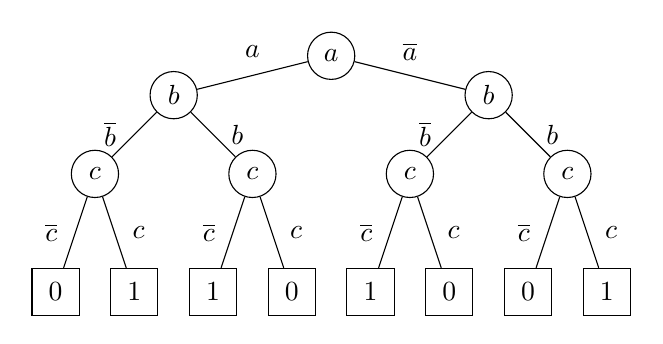
\begin{tikzpicture}
	[minimum size=6mm,
	 inner sep=1mm,
	 level/.style={sibling distance=8cm/(2^(#1)),
	 	level distance=.5cm*#1}]
	 
  \node (a) [knoten] {$a$}
  	child { node (b1) [knoten] {$b$}
  		child { node (c1) [knoten] {$c$}
  			child { node (l1) [blatt] {0} edge from parent node [left] {$\overline{c}$} }
  			child { node (l2) [blatt] {1} edge from parent node [right] {$c$} }
  			edge from parent node [left] {$\overline{b}$}
  		}
  		child { node (c2) [knoten] {$c$}
  			child { node (l3) [blatt] {1} edge from parent node [left] {$\overline{c}$} }
  			child { node (l4) [blatt] {0} edge from parent node [right] {$c$} }
  			edge from parent node [right] {$b$} 
  		}
  		edge from parent node [left, above] {$a$}
  	}
  	child { node (b2) [knoten] {$b$}
  		child { node (c3) [knoten] {$c$}
  			child { node (l5) [blatt] {1} edge from parent node [left] {$\overline{c}$} }
  			child { node (l6) [blatt] {0} edge from parent node [right] {$c$} }
  			edge from parent node [left] {$\overline{b}$} 
  		}
  		child { node (c3) [knoten] {$c$}
  			child { node (l7) [blatt] {0} edge from parent node [left] {$\overline{c}$} }
  			child { node (l8) [blatt] {1} edge from parent node [right] {$c$} }
  			edge from parent node [right] {$b$} 
  		}
  		edge from parent node [right, above] {$\overline{a}$}
  	};
\end{tikzpicture}
\caption{Beispiel eines binären Entscheidungsdiagramms}
\label{EntscheidungsdiagrammBsp}
\end{figure}

Der Entscheidungsbaum kann durch Verschmelzen gleicher Teilbäume und durch Löschen von irrelevanten Knoten reduziert werden. Zwei Teilbäume können miteinander verschmolzen werden, wenn sie gleich sind. Um die Übersicht zu behalten bietet es sich an möglichst große Teilbäume zu verschmelzen. Abbildung \ref{verschmelzung} zeigt dies anhand des oben angegebenen Beispiels.
\begin{figure}[hp]
\label{verschmelzung}
\centering
\caption{Reduktion eines Entscheidungsdiagramms mittels Verschmelzung}
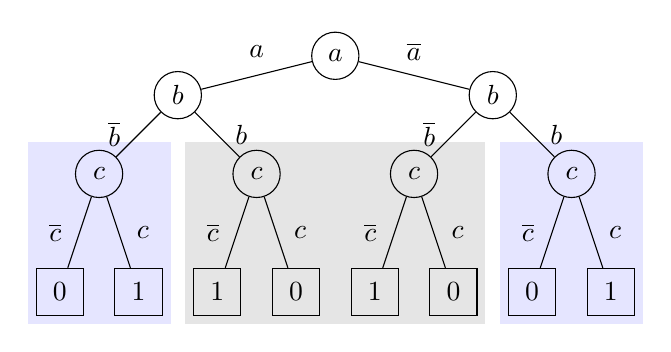
\begin{tikzpicture}
	[minimum size=6mm,
	 inner sep=1mm,
	 level/.style={sibling distance=8cm/(2^(#1)),
	 	level distance=.5cm*#1}]
	 
  \node (a) [knoten] {$a$}
  	child { node (b1) [knoten] {$b$}
  		child { node (c1) [knoten] {$c$}
  			child { node (l1) [blatt] {0} edge from parent node [left] {$\overline{c}$} }
  			child { node (l2) [blatt] {1} edge from parent node [right] {$c$} }
  			edge from parent node [left] {$\overline{b}$}
  		}
  		child { node (c2) [knoten] {$c$}
  			child { node (l3) [blatt] {1} edge from parent node [left] {$\overline{c}$} }
  			child { node (l4) [blatt] {0} edge from parent node [right] {$c$} }
  			edge from parent node [right] {$b$} 
  		}
  		edge from parent node [left, above] {$a$}
  	}
  	child { node (b2) [knoten] {$b$}
  		child { node (c3) [knoten] {$c$}
  			child { node (l5) [blatt] {1} edge from parent node [left] {$\overline{c}$} }
  			child { node (l6) [blatt] {0} edge from parent node [right] {$c$} }
  			edge from parent node [left] {$\overline{b}$} 
  		}
  		child { node (c4) [knoten] {$c$}
  			child { node (l7) [blatt] {0} edge from parent node [left] {$\overline{c}$} }
  			child { node (l8) [blatt] {1} edge from parent node [right] {$c$} }
  			edge from parent node [right] {$b$} 
  		}
  		edge from parent node [right, above] {$\overline{a}$} % right, above could also be realized with xshift=10pt and yshift=10pt
  	};
  	
  \begin{pgfonlayer}{background}
  	\node [rectangle, fill=black!10!white, fit=(c2)(l3)(l6)] {};
  	\node [rectangle, fill=blue!10!white, fit=(c1)(l1)(l2)] {};
  	\node [rectangle, fill=blue!10!white, fit=(c4)(l7)(l8)] {};
	\end{pgfonlayer}
\end{tikzpicture}

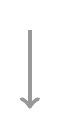
\begin{tikzpicture}
	\draw[ultra thick, color=black!40!white, ->] (0,0) -- (0,-1); 
\end{tikzpicture}

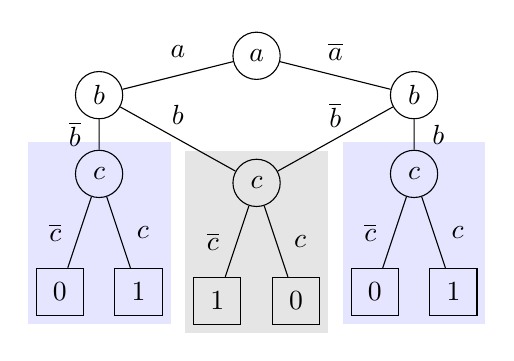
\begin{tikzpicture}
	[graph,
	 level/.style={sibling distance=8cm/(2^(#1)),
	 	level distance=.5cm*#1}]
	 
  \node (a) [knoten] {$a$}
  	child { node (b1) [knoten] {$b$}
  		child { node (c1) [knoten] {$c$}
  			child { node (l1) [blatt] {0} edge from parent node [left] {$\overline{c}$} }
  			child { node (l2) [blatt] {1} edge from parent node [right] {$c$} }
  			edge from parent node [left] {$\overline{b}$}
  		}
  		edge from parent node [left, above] {$a$}
  	}
  	child { node (b2) [knoten] {$b$}
  		child { node (c4) [knoten] {$c$}
  			child { node (l7) [blatt] {0} edge from parent node [left] {$\overline{c}$} }
  			child { node (l8) [blatt] {1} edge from parent node [right] {$c$} }
  			edge from parent node [right] {$b$} 
  		}
  		edge from parent node [right, above] {$\overline{a}$} % right, above could also be realized with xshift=10pt and yshift=10pt
  	};
  	
  	\node (c2) [knoten, below=of a] {$c$}
			child[sibling distance=1cm, level distance=1.5cm] { node (l3) [blatt] {1} edge from parent node [left] {$\overline{c}$} }
			child[sibling distance=1cm, level distance=1.5cm] { node (l4) [blatt] {0} edge from parent node [right] {$c$} }
			edge node[above] {$b$} (b1) 
			edge node[above] {$\overline{b}$} (b2);
  	
  \begin{pgfonlayer}{background}
  	\node [rectangle, fill=black!10!white, fit=(c2)(l3)(l4)] {};
  	\node [rectangle, fill=blue!10!white, fit=(c1)(l1)(l2)] {};
  	\node [rectangle, fill=blue!10!white, fit=(c4)(l7)(l8)] {};
	\end{pgfonlayer}
\end{tikzpicture}

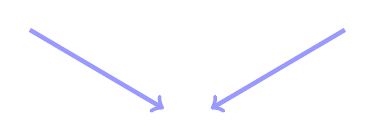
\begin{tikzpicture}
	\draw[ultra thick, color=blue!40!white, ->] (-2,0) -- (-.3,-1); 
	\draw[ultra thick, color=blue!40!white, ->] (2,0) -- (.3,-1); 
\end{tikzpicture}

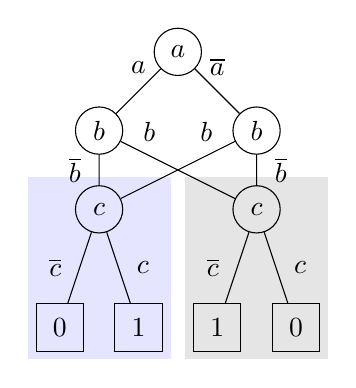
\begin{tikzpicture}
	[graph,
	 level 1/.style={sibling distance=2cm, level distance=1cm},
	 level 2/.style={sibling distance=2cm, level distance=1cm},
	 level 3/.style={sibling distance=1cm, level distance=1.5cm}]
	 
  \node (a) [knoten] {$a$}
  	child { node (b1) [knoten] {$b$}
  		child { node (c1) [knoten] {$c$}
  			child { node (l1) [blatt] {0} edge from parent node [left] {$\overline{c}$} }
  			child { node (l2) [blatt] {1} edge from parent node [right] {$c$} }
  			edge from parent node [left] {$\overline{b}$}
  		}
  		edge from parent node [left, above] {$a$}
  	}
  	child { node (b2) [knoten] {$b$}
  		child { node (c2) [knoten] {$c$}
  			child { node (l3) [blatt] {1} edge from parent node [left] {$\overline{c}$} }
  			child { node (l4) [blatt] {0} edge from parent node [right] {$c$} }
  			edge from parent node [right] {$\overline{b}$} 
  		}
  		edge from parent node [right, above] {$\overline{a}$} % right, above could also be realized with xshift=10pt and yshift=10pt
  	};
  	
  	\draw (b1) to node [near start, above] {$b$} (c2);
  	\draw (b2) to node [near start, above] {$b$} (c1);
  	
  	\begin{pgfonlayer}{background}
  	\node [rectangle, fill=black!10!white, fit=(c2)(l3)(l4)] {};
  	\node [rectangle, fill=blue!10!white, fit=(c1)(l1)(l2)] {};
	\end{pgfonlayer}
\end{tikzpicture}

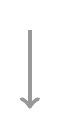
\begin{tikzpicture}
	\draw[ultra thick, color=black!40!white, ->] (0,0) -- (0,-1); 
\end{tikzpicture}

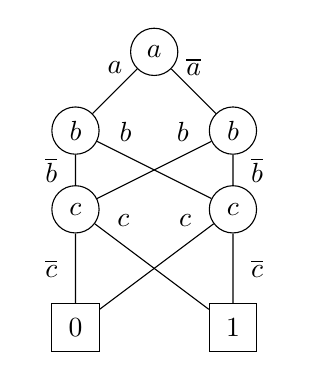
\begin{tikzpicture}
	[graph,
	 level 1/.style={sibling distance=2cm, level distance=1cm},
	 level 2/.style={sibling distance=2cm, level distance=1cm},
	 level 3/.style={sibling distance=1cm, level distance=1.5cm}]
	 
  \node (a) [knoten] {$a$}
  	child { node (b1) [knoten] {$b$}
  		child { node (c1) [knoten] {$c$}
  			child { node (l1) [blatt] {0} edge from parent node [left] {$\overline{c}$} }
  			edge from parent node [left] {$\overline{b}$}
  		}
  		edge from parent node [left, above] {$a$}
  	}
  	child { node (b2) [knoten] {$b$}
  		child { node (c2) [knoten] {$c$}
  			child { node (l2) [blatt] {1} edge from parent node [right] {$\overline{c}$} }
  			edge from parent node [right] {$\overline{b}$}
  		}
  		edge from parent node [right, above] {$\overline{a}$} % right, above could also be realized with xshift=10pt and yshift=10pt
  	};
  	
  	\draw (b1) to node [near start, above] {$b$} (c2);
  	\draw (b2) to node [near start, above] {$b$} (c1);
  	
  	\draw (c1) to node [near start, above] {$c$} (l2);
  	\draw (c2) to node [near start, above] {$c$} (l1);
\end{tikzpicture}
\end{figure}

Führen die beiden ausgehenden Kanten eines Knotens auf denselben Knoten oder dasselbe Blatt so kann der Knoten gelöscht werden und dessen eingehende Kanten auf das Kind des gelöschten Knotens verzweigt werden. 
\begin{figure}[hp]
\centering
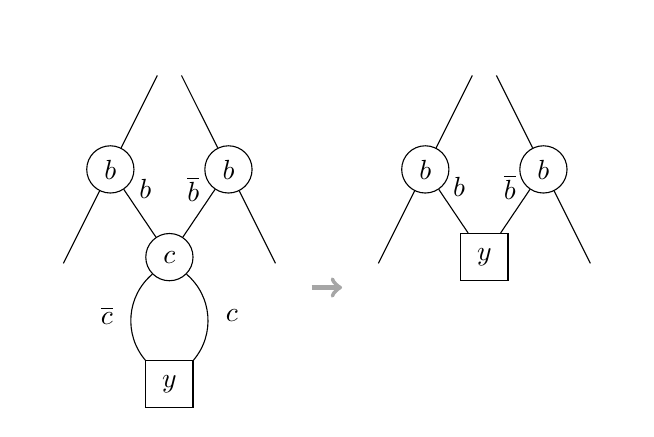
\begin{tikzpicture}[graph, bend angle=45]
	\node[] (a) {}
	  child{ node[knoten] (b1) {$b$}
	  	child{ node (c1) {} }
	  	child[missing]{} }
		child{ node[knoten] (b2) {$b$}
	  	child[missing]{}
	  	child{ node (c2) {} } };
	\node[knoten, below=of a, yshift=-1cm] (c) {$c$}
		edge node[right, above, xshift=0.7mm] {$b$} (b1)
		edge node[left, above, xshift=-0.7mm] {$\overline{b}$}(b2);
	\node[blatt, below=of c] {$y$}
		edge[bend left] node[left] {$\overline{c}$} (c)
		edge[bend right] node[right] {$c$} (c);
		
	\begin{scope}[xshift=4cm]
		\node[] (a') {}
		  child{ node[knoten] (b1') {$b$}
		  	child{ node (c1') {} }
		  	child[missing]{} }
			child{ node[knoten] (b2') {$b$}
		  	child[missing]{}
		  	child{ node (c2') {} } };
		\node[blatt, below=of a', yshift=-1cm] (c') {$y$}
			edge node[right, above, xshift=0.7mm] {$b$} (b1')
			edge node[left, above, xshift=-0.7mm] {$\overline{b}$}(b2');
	\end{scope}
	
	\draw[->, ultra thick, color=black!35] (c2) to (c1');
\end{tikzpicture}
\caption{Löschen eines Knotens}
\end{figure}

\section{Quine-McCluskey-Verfahren}
Nach dem Quine-McCluskey-Verfahren können systematisch Terme zusammengefasst werden, welche sich durch Negation einer einzigen Variablen unterscheiden. Das Quine-McCluskey-Verfahren eignet sich im Gegensatz zu KV-Diagrammen für Funktionen mit beliebig vielen Eingangsvariablen. Außerdem ist es leicht zu automatisieren. Beim händischen Minimieren von Funktionen sollten für Funktionen mit 4 oder weniger Eingangsvariablen KV-Diagramme verwendet werden, da diese übersichtlicher und für uns Menschen leichter zu lösen sind. Für Funktionen mit mehr als 4 Eingangsvariablen sollte das Quine-McCluskey-Verfahren eingesetzt werden.

Die Vereinfachung geschieht mittels Ordnungstabellen, welche schrittweise reduziert werden. 
\begin{enumerate}
  \item Die Minterme der Funktion werden aufgrund der Anzahl affirmierter\footnote{Die Affirmation ist das Gegenteil der Negation. Eine affirmierte Variable ist also eine Variable als solche.} Variablen zusammengefasst. So entstehen Gruppen von Termen, wobei alle Terme einer jeweiligen Gruppe gleich viele affirmierte Variablen besitzen. Die so entstandene Ordnung lässt sich in einer Ordnungstabelle notieren, wobei die Gruppen nach Anzahl der affirmierten Variablen aufsteigend sortiert werden.
  \item Anschließend werden jeweils zwei Gruppen zusammengefasst, welche in der Sortierung direkt nebeneinander stehen. Eine Zusammenfassung zweier Terme wird vollzogen, wenn die Terme sich in ausschließlich einer Stelle durch Affirmation und Negation derselben Stelle unterscheiden. Die zusammengefassten Terme werden wiederum neuen Gruppen zugeordnet und in einer Ordnungstabelle nach gleichem Schema notiert. So entstehen Tabellen höherer Ordnung bis keine weitere Zusammenfassung möglich ist.
  \item Terme, welche nicht weiter zusammengefasst werden konnten werden aufgrund dieser Eigenschaft Primimplikanten genannt. Für die minimierte Funktion sind allerdings nicht zwingend alle Primimplikanten notwendig. Primimplikanten, welche für die Funktion notwendig sind, werden Kernimplikanten genannt. Die Kernimplikanten werden anhand der Primimplikantentafel bestimmt. Dabei muss jeder Minterm von mindestens einem Kernimplikanten abgedeckt sein. Es gilt also eine minimale Anzahl an Kernimplikanten zu bestimmen, wobei jeder Minterm über die Menge der ausgewählten Kernimplikanten abgedeckt sein muss.
\end{enumerate}

Beispiel: Die Funktion f mit den vier Eingangsvariablen $a$, $b$, $c$ und $d$ sei durch ihre Minterme $\{m_i \mid i \in {0,2,5,8,10,12,13,15}\}$ eindeutig bestimmt.
$$ f(a,b,c,d) = \overline{a}\overline{b}\overline{c}\overline{d} + \overline{a}b\overline{c}\overline{d} + a\overline{b}c\overline{d} + \overline{a}\overline{b}\overline{c}d + \overline{a}b\overline{c}d + \overline{a}\overline{b}cd + a\overline{b}cd + abcd$$
\begin{center}
Die Ordnungstabelle 0-ter Ordnung ist:

\begin{tabular}{c *{4}{c} c l}
Term & \multicolumn{4}{c}{Belegung} & Gruppe & Notiz \\
     & $a$ & $b$ & $c$ & $d$        &        &       \\ \hline
 0   & $0$ & $0$ & $0$ & $0$        & 0      &       \\ \hline
 2   & $0$ & $1$ & $0$ & $0$        & 1      &       \\
 8   & $0$ & $0$ & $0$ & $1$        &        &       \\ \hline
 5   & $1$ & $0$ & $1$ & $0$        & 2      &       \\
10   & $0$ & $1$ & $0$ & $1$        &        &       \\
12   & $0$ & $0$ & $1$ & $1$        &        &       \\ \hline
13   & $1$ & $0$ & $1$ & $1$        & 3      &       \\ \hline
15   & $1$ & $1$ & $1$ & $1$        & 4      &       \\
\end{tabular} 
\end{center}

\begin{center}
Die Ordnungstabelle 1-ter Ordnung ist:

\begin{tabular}{c *{4}{c} c l}
Term  & \multicolumn{4}{c}{Belegung} & Gruppe & Notiz \\
      & $a$ & $b$ & $c$ & $d$        &        &       \\ \hline
 0,2  & $0$ & $-$ & $0$ & $0$        & 0      &       \\ 
 0,8  & $0$ & $0$ & $0$ & $-$        &        &       \\ \hline
 2,10 & $0$ & $1$ & $0$ & $-$        & 1      &       \\ 
 8,10 & $0$ & $-$ & $0$ & $1$        &        &       \\
 8,12 & $0$ & $0$ & $-$ & $1$        &        & prim  \\ \hline
 5,13 & $1$ & $0$ & $1$ & $-$        & 2      & prim  \\ 
12,13 & $-$ & $0$ & $1$ & $1$        &        & prim  \\ \hline
13,15 & $1$ & $-$ & $1$ & $1$        & 3      & prim  \\
\end{tabular} 
\end{center}

\begin{center}
Die Ordnungstabelle 2-ter Ordnung ist:

\begin{tabular}{c *{4}{c} c l}
	Term       & \multicolumn{4}{c}{Belegung} & Gruppe & Notiz \\
	~          & a   & b   & c   & d   & ~    & ~              \\ \hline
	$0,2,8,10$ & $-$ & $0$ & $-$ & $0$ & $0$  & prim           \\
	$0,8,2,10$ & $-$ & $0$ & $-$ & $0$ & ~    & streichen      \\
\end{tabular}
\end{center}

\begin{center}
die Primimplikantentafel ist also:
\begin{tabular}{l|*{8}{l|}l}
                & \multicolumn{8}{c|}{Minterme}                       & ~     \\
  Primimplikant & 0    & 2    & 5    & 8    & 10   & 12 & 13   & 15   & ~     \\ \hline
  $8,12$        & ~    & ~    & ~    & + *  & ~    & +  & ~    & ~    & $P_1$ \\
  $5,13$        & ~    & ~    & + \# & ~    & ~    & ~  & + *  & ~    & $K_1$ \\
  $12,13$       & ~    & ~    & ~    & ~    & ~    & +  & + *  & ~    & $P_2$ \\
  $13,15$       & ~    & ~    & ~    & ~    & ~    & ~  & + \# & + \# & $K_2$ \\
  $0,2,8,10$    & + \# & + \# & ~    & + \# & + \# & ~  & ~    & ~    & $K_3$ \\
\end{tabular}
\end{center}
Die Minterme $m_0$, $m_5$, $m_8$, $m_{10}$, $m_{13}$ und $m_{15}$ werden über die Terme $K_1$, $K_2$ und $K_3$ abgedeckt. Wie an der Tafel zu erkennen ist, kann der Minterm $m_{12}$ von $P_1$ oder $P_2$ abgedeckt werden. Daher muss einer der beiden Terme als Kernimplikant gewählt werden. Es gibt also zwei mögliche minimierte Formen der Funktion:
\begin{align*}
	f(a,b,c,d) &= \overline{a}\overline{b}\overline{c}\overline{d} + \overline{a}b\overline{c}\overline{d} 
	              + a\overline{b}c\overline{d} + \overline{a}\overline{b}\overline{c}d + \overline{a}b\overline{c}d 
	              + \overline{a}\overline{b}cd + a\overline{b}cd + abcd \\
	           &= \overline{a}\overline{b}d + a\overline{b}c + acd + \overline{b}\hspace{2pt}\overline{d} \\
	           &= \overline{b}cd + a\overline{b}c + acd + \overline{b}\hspace{2pt}\overline{d} \\
\end{align*}









 %%\documentclass[11pt,a4paper]{scrartcl}
%\documentclass[11pt,a4paper]{scrreprt}
\documentclass[11pt,a4paper,oneside]{scrbook}
%\documentclass[11pt,a4paper,oneside,draft]{scrbook}

\usepackage[utf8]{inputenc}
\usepackage[T1]{fontenc}
\usepackage{lmodern}
\usepackage{ngerman}

\usepackage{amsmath} % align

\usepackage[pdftex]{graphicx}
\graphicspath{{../Abbildungen_export/}, {../../Abbildungen_export/}}

\usepackage{tikz}
\usetikzlibrary{positioning, backgrounds, fit, calc}
\tikzset{knoten/.style={circle,draw,thin},
	blatt/.style={rectangle,draw,thin},
	graph/.style={minimum size=6mm, inner sep=1mm},
	gatter/.style={minimum width=10mm, minimum height=15mm},
	helper/.style={inner sep=0} }

\usepackage{wasysym}

\definecolor{myLinkColor}{rgb}{0.25882353,0.36470588,0.60392157}
\usepackage[
    pdftex,
    a4paper,
    bookmarks,
    bookmarksopen=true,
    bookmarksnumbered=true,
    pdfauthor={Kajetan Weiß},
    pdftitle={Digitaltechnik Aufarbeitung},
    colorlinks,
    linkcolor=myLinkColor,
    urlcolor=myLinkColor
]{hyperref}

% usefull commands: \hspace{-\parindent}
 \begin{document}

\chapter{Schaltnetzrealisierung}
Schaltnetze können systematisch über ein Binary Decision Diagram oder einer Schaltfunktion umgesetzt werden. 
%TODO SN-Realisierung mit Schaltdiagrammen ausführen 
{\sc nand} bzw. {\sc nor} Schaltkreise sind dabei physikalisch günstiger, da weniger Transistoren, Leistung und geringere Schaltzeiten benötigt werden. Näheres zu {\sc nand}/{\sc nor} Funktionen ist im Dokument Digitaltechnik Aufbereitung zu finden. 

\section{{\sc {\sc nand}} und {\sc nor} Formen}
Jede Schaltfunktion kann nach den Gesetzen von De Morgan mit {\sc nand} oder {\sc nor} Bausteinen umgesetzt werden. Dabei wird der Umstand genutzt, dass die doppelte Negation die ursprünglche Aussage erhält. Im Folgenden ein Beispiel:
\begin{align*}
y &= a \cdot b + \overline{c} \cdot d \\
  &= \overline{\overline{a \cdot b + \overline{c} \cdot d}} 
  	\textnormal{ \# doppelte Negation erhält die Aussage} \\
  &= \overline{\overline{a \cdot b} \cdot \overline{\overline{c} \cdot d}}
  \textnormal{ \# Gesetz von De Morgan führt zu {\sc nand}} \\
  &= \overline{\overline{\overline{\overline{a \cdot b} \cdot \overline{\overline{c} \cdot d}}}} 
  	\textnormal{ \# Doppelte Negation für {\sc nor} Realisierung} \\ 
  &= \overline{\overline{\overline{a \cdot b} + \overline{\overline{c} \cdot d}}} \\
  &= \overline{\overline{\overline{a \cdot b} + \overline{\overline{c} \cdot d}}} \\
  &= \overline{\overline{(\overline{a} + \overline{b}) + (c + \overline{d})}} \textnormal{ \# {\sc nor} Realisierung}\\
  &= \overline{\overline{\overline{\overline{(\overline{a} + \overline{b})}} 
  	+ \overline{\overline{(c + \overline{d})}}}} \\
\end{align*}

Ausgehend von einer Disjunktiven Form\footnote{Näheres zu Disjunktiven Formen kann im Dokument Digitaltechnik Aufarbeitung nachgeschlagen werden.} kann also über die Doppelte Negation zu einer {\sc nand} Funktion umgebaut werden. Es gilt mit den Mintermenen $m_i$:

\begin{align*}
	y &= m_1 + m_2 + \ldots + m_n = \sum_{i=1}^n m_i \\
	  &= \overline{\overline{m_1 + m_2 + \ldots + m_n}} = \overline{\overline{\sum_{i=1}^n m_i}} \\
	  &= \overline{\overline{m_1} \cdot \overline{m_2} \cdot \overline{(\ldots)} \cdot \overline{m_n}} 
	   = \overline{\prod_{i=1}^n \overline{m_i}} \\
\end{align*}
Als allgemeine Methode um von einer Disjunktiven Form zu einer {\sc nand} Form umzuformen kann angegeben werden:
\begin{enumerate}
  \item erhalte Aussage mittels doppelter Negation
  \item wende ein mal das Gesetz von De Morgan an
  \item Ergebnis ist eine zweistufige {\sc nand} Form der Funktion
\end{enumerate}
Ein Beispiel zur Überführung der Form einer Funktion in Disjunktiver Form zu einer {\sc nand} Form: 
\begin{align*}
	y &= ab + \overline{c}d + e \\
	  &= \overline{\overline{ab + \overline{c}d + e}} \\
	  &= \overline{\overline{a}\overline{b} \cdot c\overline{d} \cdot \overline{e}} \\
\end{align*}
%TODO schaltdiagramm ergänzen

Um die Umformung einer Disjunktiven Form auf eine {\sc nor} Form zu realisieren können folgende Regeln genutzt werden:
\begin{align*}
	y = \sum_{i=1}^n m_i = \sum_{i=1}^n \overline{\overline{m_i}} 
		= \overline{\overline{\sum_{i=1}^n \overline{\overline{m_i}}}} \\
\end{align*}
Als allgemeine Methode um von einer Disjunktiven Form zu einer {\sc nand} Form umzuformen kann angegeben werden:
\begin{enumerate}
  \item erhalte Aussage mittels doppelter Negation der gesamten Funktion
  \item erhalte die Aussage jedes Minterms mittels doppelter Negation des jeweiligen Terms
  \item wende ein mal das Gesetz von De Morgan auf jeden doppelt negierten Minterm an
  \item Ergebnis ist eine dreistufige {\sc nor} Form der Funktion
\end{enumerate}
Ein Beispiel zur Überführung einer Disjunktiver Form zu einer {\sc nor} Form: 
\begin{align*}
	y &= ab + \overline{c}d + e \\
	  &= \overline{\overline{\overline{\overline{ab}} + \overline{\overline{\overline{c}d}} 
	  	+ \overline{\overline{e}}}} \\	  
	  &= \overline{\overline{\overline{(\overline{a} + \overline{b})} + \overline{(c + \overline{d})} + e}} \\
\end{align*}
%TODO schaltdiagramm ergänzen

Ausgehend von einer Konjunktiven Form mit den Maxtermen $M_i$ kann eine \textsc{nor} Form mit folgenden Regeln erstellt werden:
\begin{align*}
	y = \prod_{i=1}^n M_i = \overline{\overline{\prod_{i=1}^n M_i}} = \overline{\sum_{i=1}^n \overline{M_i}} \\
\end{align*}
Als allgemeine Methode um von einer Konjunktiven Form zu einer {\sc nor} Form umzuformen kann angegeben werden:
\begin{enumerate}
  \item erhalte Aussage mittels doppelter Negation
  \item wende ein mal das Gesetz von De Morgan an
  \item Ergebnis ist eine zweistufige {\sc nor} Form der Funktion
\end{enumerate}
Ein Beispiel zur Überführung der Form einer Funktion in Konjunktiver Form zu einer {\sc nor} Form: 
\begin{align*}
	y &= (a + b) \cdot (\overline{c} + d) \cdot e \\
	  &= \overline{\overline{(a + b) \cdot (\overline{c} + d) \cdot e}} \\
	  &= \overline{\overline{(a + b)} + \overline{(\overline{c} + d)} + \overline{e}} \\
\end{align*}
%TODO schaltdiagramm ergänzen

Ausgehend von einer Konjunktiven Form mit den Maxtermen $M_i$ kann eine \textsc{nand} Form mit folgenden Regeln erstellt werden:
\begin{align*}
	y = \prod_{i=1}^n M_i = \overline{\overline{\prod_{i=1}^n M_i}} 
		= \overline{\overline{\sum_{i=1}^n \overline{\overline{M_i}}}} \\
\end{align*}
Als allgemeine Methode um von einer Konjunktiven Form zu einer {\sc nand} Form umzuformen kann angegeben werden:
\begin{enumerate}
  \item erhalte Aussage mittels doppelter Negation
  \item erhalte die Aussage jedes Maxterms mittels doppelter Negation des jeweiligen Terms
  \item wende ein mal das Gesetz von De Morgan auf jeden doppelt negierten Maxterm an
  \item Ergebnis ist eine dreistufige {\sc nand} Form der Funktion
\end{enumerate}
Ein Beispiel zur Überführung der Form einer Funktion in Konjunktiver Form zu einer {\sc nand} Form: 
\begin{align*}
	y &= (a + b) \cdot (\overline{c} + d) \cdot e \\
	  &= \overline{\overline{\overline{\overline{(a + b)}} \cdot \overline{\overline{(\overline{c} + d)}} 
	  	\cdot \overline{\overline{e}}}} \\
	  &= \overline{\overline{\overline{(\overline{a} \cdot \overline{b})} 
	  	\cdot \overline{(c \cdot \overline{d})} \cdot e}} \\	  
\end{align*}
%TODO schaltdiagramm ergänzen

\section{Positive und Negative Logik}
Um die binären Werte $\{0, 1\}$ technisch abbilden zu können werden in der Halbleitertechnik die Signalpegel Low (L) und High (H) verwendet. Die Zuordnung von Signalpegel auf binären Wert ist dabei frei wählbar. Allerdings wirkt die Zuordnung sich auf die Logik aus. Tabelle \ref{posNegLogik} zeigt die Standard-Zuordnung der Signalpegel für die logische Grundfunktion. Je nachdem ob L $\mapsto$ 0 oder L $\mapsto$ 1 zugeordnet wird ergibt sich für die Standard-Zuordnung entweder das logische {\sc and} oder {\sc or}.
\begin{table}[h]
\centering
\begin{tabular}{*{2}{cc|c||}cc|c}
\multicolumn{3}{c||}{Signalpegel} & \multicolumn{6}{c}{Schaltfunktion}\\
\multicolumn{3}{c||}{Standard Zuordnung} & \multicolumn{3}{c||}{positive Logik: {\sc and}} & \multicolumn{3}{c}{negative Logik: {\sc or}}\\
\multicolumn{3}{c||}{\{L, H\} $\mapsto$ \{L, H\}} & \multicolumn{3}{c||}{L $\mapsto$ 0} & \multicolumn{3}{c}{L $\mapsto$ 1}\\ \hline
b & a & y & b & a & y & b & a & y \\ \hline
L & L & L & 0 & 0 & 0 & 1 & 1 & 1 \\
L & H & L & 0 & 1 & 0 & 1 & 0 & 1 \\
H & L & L & 1 & 0 & 0 & 0 & 1 & 1 \\
H & H & H & 1 & 1 & 1 & 0 & 0 & 0 \\
\end{tabular}
\caption{Positive und Negative Logik}
\label{posNegLogik}
\end{table}

Aufgrund dieser Zusammenhänge wird die positive Logik auch {\sl wired {\sc and}} und die negative Logik auch {\sl wired {\sc or}} genannt.  
  
\section{Multiplexer}  
Mit Multiplexern kann von mehreren Eingängen einer geziehlt per Addressierung ausgewählt werden. Diese Funktion kommt beispielsweise in Bus-Systemen zum Einsatz. Je nachdem wieviele Werte addressiert werden sollen, müssen entsprechend viele Variablen als Adressvariablen gewählt werden. Jede Adressvariable steht dabei für eine Stelle einer Adresse. 

Ein 2 zu 1 Multiplexer hat demnach zwei Eingänge, die es zu addressieren gilt. Demnach muss eine zusätzliche Eingangsvariable als Addressvariable zur Darstellung der Addressen 0 und 1 ergänzt werden. Abbildung \ref{2zu1MuxReal} zeigt die Realisierung eines 2 zu 1 Multiplexers. Hat $a$ den Wert 0 so wird der Wert $x_0$ an y übertragen. Hat $a$ den Wert 1 wird der Wert von $x_1$ ausgewählt und an $y$ übertragen.
\begin{figure}[htp]
	\centering
	\includegraphics[scale=1]{2zu1MuxRealisierung.pdf}
	\caption{Schaltbild eines 2 zu 1 Multiplexers}
	\label{2zu1MuxReal}
\end{figure}

Um die Beschreibung von Multiplexern zu vereinfachen kann die Notation aus Abbildung \ref{MulNot} verwendet werden.
\begin{figure}[htp]
	\centering
	\includegraphics[scale=1]{MultiplexerNotation.pdf}
	\caption{Notation eines n zu 1 Multiplexers}
	\label{MulNot}
\end{figure}

Nach demselben Schema lassen sich $n$ zu 1 Multiplexer aufbauen. Wobei $n$ die Anzahl addressierbarer Elemente ist. Praktisch angewandt kann dies Beispielsweise für eine Register zu Bus Verbindung genutzt werden. Wenn der Wert eines Registers einem Bus übergeben werden soll geschieht folgendes: In die Adressvariablen wird die Adresse des Registers geschrieben. Damit wird im Multiplexer das entsprechende Register ausgewählt. Die Ausgangsvariable erhält somit den Wert des Registers. Abbildung \ref{4zu1MuxReal} zeigt das Schaltbild eines 4 zu 1 Multiplexers.

\begin{figure}[htp]
	\centering
	\includegraphics[scale=1]{4zu1MuxRealisierung.pdf}
	\caption{Schaltbild eines 4 zu 1 Multiplexers}
	\label{4zu1MuxReal}
\end{figure}

\begin{figure}
	\centering
	\includegraphics[scale=1]{4zu1Mux.pdf}
	\caption{Kurznotation des 4 zu 1 Multiplexers}
\end{figure}

Aufgrund dieser zuordnenden Eigenschaft können Multiplexer auch zur Realisierung von Schaltfunktionen verwendet werden. Zu diesem Zweck werden den Addressen die Funktionswerte der zu realisierenden Funktion zugeordnet. Die Addressen entsprechen somit den Belegungen der Eingangsvariablen der Funktion in Disjunktiver Normalform. Da die Disjunktive Normalform aus der Schaltbelegungstabelle abgelesen werden kann, können die Funktionswerte aus der Schaltbelegungstabelle direkt auf den Multiplexer übertragen werden. Abbildung \ref{FunMuxBsp} zeigt ein Beispiel einer Funktion und deren Darstellung in einer Schaltbeleungstabelle, als Disjunktive Normalform und realisiert als Multiplexer.
\begin{table}[htp]
	\centering
	\begin{tabular}{*{9}{l}}    
	$i$ & 0 & 1 & 2 & 3 & 4 & 5 & 6 & 7 \\ \hline
	$c$ & 0 & 0 & 0 & 0 & 1 & 1 & 1 & 1 \\
	$b$ & 0 & 0 & 1 & 1 & 0 & 0 & 1 & 1 \\
	$a$ & 0 & 1 & 0 & 1 & 0 & 1 & 0 & 1 \\ \hline
	$y$ & 1 & 0 & 1 & 0 & 1 & 0 & 0 & 1 \\
	\end{tabular}
\end{table}
$$ y = \overline{a}\overline{b}\overline{c} + \overline{a}b\overline{c} + \overline{a}\overline{b}c + abc $$
\begin{figure}[htp]	
	\centering
	\includegraphics{8zu1MuxFunBsp.pdf}
	\caption{Beispiel einer Funktion Realisiert als Multiplexer}
	\label{FunMuxBsp}
\end{figure}

Bei der Realiserung von Funktionen als Multiplexer können die Addressvariablen zur Minimierung des Multiplexers dienen. Dazu werden die Werte des Multiplexers abhängig von den Eingangsvariablen gesetzt. Mit diesem Verfahren kann die Funktion aus \ref{FunMuxBsp} mit dem Multiplexer aus Abbildung \ref{minMuxFunBsp} realisiert werden.

\begin{figure}[htp]
	\centering
	\begin{tabular}{*{9}{l}}    
	$i$ & 0 & 1 & 2 & 3 & 4 & 5 & 6 & 7 \\ \hline
	$c$ & 0 & 0 & 0 & 0 & 1 & 1 & 1 & 1 \\
	$b$ & 0 & 0 & 1 & 1 & 0 & 0 & 1 & 1 \\
	$a$ & 0 & 1 & 0 & 1 & 0 & 1 & 0 & 1 \\ \hline
	$y$ & 1 & 0 & 1 & 0 & 1 & 0 & 0 & 1 \\
	\end{tabular}
	$\mapsto$
	\begin{tabular}{*{5}{l}}    
	$b$ & 0 & 0 & 1              & 1 \\
	$a$ & 0 & 1 & 0              & 1 \\ \hline
	$y$ & 1 & 0 & $\overline{c}$ & $c$ \\
	\end{tabular}
	
	\vspace{1cm}
	
	\includegraphics{4zu1minMuxFunBsp.pdf}
	\caption{Minimierter Multiplexer}
	\label{minMuxFunBsp}
\end{figure} 

%TODO Abschnitt "Demultiplexer" aus DgS-SN-2f ergänzen 

\section{{\sc Rom, Prom}-Realisierung einer Schaltfunktion}
{\sc Rom} steht für Read Only Memory. {\sc Prom} steht entsprechend für Programmable Read Only Memory. Es handelt sich um unversell einsetzbare addressierende Einheiten zur Realisierung von Schaltnetzen. Jeder Addresse wird hierbei ein Speicherwort als Festwert bzw. Konstante zugeordnet. So können allen Variablenbelegungen einer Funktion der entsprechende Wert als Speicherwort im {\sc rom} zugeordnet werden. Dies ist Verleichbar mit dem nicht minimierten Verfahren zur Realisierung einer Funktion mit einem Multiplexer.

Beispiel: Es sei folgende Funktion gegeben:
$$f(x_0, x_1, x_2, x_3) = y = \prod \{M_0, M_2, M_3, M_4, M_5, M_8, M_{12}, M_{13}\}$$ %führt zu Anzeigefehler?
Die Funktion soll mit einem {\sc prom} realisiert werden. Es werden also vier Addresseingänge benötigt, womit $2^4$ Werte addressiert werden können. An den jeweiligen Addressen, die den Indizes der Maxterme entsprechen, wird der Wert $0$ einprogrammiert. An allen übrigen Addressen wird der Wert $1$ einprogrammiert, da diese Addressen den Mintermen der Funktion entsprechen. Abbildung \ref{PROMbeispiel} zeigt das Schaltdiagramm für den {\sc prom}-Baustein.
\begin{figure}[htp]
%TODO SBT einfügen
	\centering
	\includegraphics{PROMbsp.pdf}
	\caption{{\sc Prom} realisiert die angegebene Schaltfunktion}
	\label{PROMbeispiel}
\end{figure}

\section{{\sc Pla}-Realisierungen}
{\sc Pla} steht für Programmable Logic Array. In einem PLA liegen alle Eingangsvariablen sowohl als solche als auch negiert vor. Die Variablenbelegungen können im Konjunktionsfeld des {\sc pla}s beliebig konjunktiv verknüpft werden. So entstehen rein konjunktiv verknüpfte Terme, welche als Minterme einer Funktion dienen können. Im Disjunktionsfeld des {\sc pla}s können die Minterme aus dem Konjunktionsfeld disjunktiv verknüpft werden. Die Verknüpfung der Variablen und Terme kann im Baustein programmiert werden. So kann jede Schaltfunktion in disjunktiver Form realisiert werden.
Da jede Variable mit jeder anderen Variablen einen Minterm bilden kann, werden genauso viele Konjunktionsbausteine benötigt, wie Eingangsvariablen vorhanden sind. Es können beliebig viele Disjunktionsbausteine im Disjunktionsfeld gewählt werden um beliebig viele Funktionen mit den im Konjunktionsfeld erstellten Mintermen zu realisieren. Abbildung \ref{PLAschem} zeigt das Schema eines {\sc pla}-Bausteins.  
\begin{figure}[htp]
	\centering
	\includegraphics[scale=1]{PLAschema.pdf}
	\caption{Schema eines {\sc pla}-Bausteins}
	\label{PLAschem}
\end{figure}

Beispiel: Die Funktionen $f, g$ und $h$ seien durch die Schaltbelegungstabelle \ref{PlaBspSBT} definiert. Die Funktion $f$ soll mittels eines {\sc pla}s realisiert werden.
\begin{table}[htp]
\centering
\begin{tabular}{*{9}{c}}
$i$ & 0 & 1 & 2 & 3 & 4 & 5 & 6 & 7 \\ \hline
$c$ & 0 & 0 & 0 & 0 & 1 & 1 & 1 & 1 \\
$b$ & 0 & 0 & 1 & 1 & 0 & 0 & 1 & 1 \\
$a$ & 0 & 1 & 0 & 1 & 0 & 1 & 0 & 1 \\ \hline
$f$ & 1 & 1 & 0 & 0 & 1 & 0 & 1 & 0 \\ \hline
$g$ & 0 & 1 & 1 & 0 & 0 & 1 & 0 & 0 \\ \hline
$h$ & 0 & 0 & 0 & 0 & 1 & 0 & 1 & 0 \\
\end{tabular}
\caption{Schaltbelegungstabelle der Funktionen $f, g$ und $h$ für das Beispiel zur Realisierung einer Funktion mittels eines {\sc pla}-Bausteins.}
\label{PlaBspSBT}
\end{table}


Die Funktionen lassen sich wie folgt minimieren:
\begin{align*}
 f &= \overline{a}c + \overline{b}\overline{c} \\
 g &= a\overline{b} + \overline{a}b\overline{c} \\
 h &= \overline{a}c \\
\end{align*}

Damit realisiert der {\sc pla}-Baustein aus Abbildung \ref{plaBeispiel} die Funktionen $f, g$ und $h$.
\begin{figure}[htp]
	\centering
	\includegraphics[scale=1]{PLAbsp.pdf}
	\caption{Beispiel eines programmierten {\sc pla}-Bausteins für die Funktionen $f, g$ und $h$ aus der Schaltbelegungstabelle \ref{PlaBspSBT}}
	\label{plaBeispiel}
\end{figure}

  
%TODO Abschnitt "Kosten" aus DgS-SN-2f ergänzen 




% \end{document}
\chapter{Laufzeitverhalten und Hazardanalyse}
Jeder Zustand den eine Schaltfunktion einnehmen kann ist fest definiert. Aus rein logischer Sicht wir einer Variablenbelegung genau ein Ergebniszustand zugeordnet. Aus praktisch physikalischer Betrachtung braucht jedes Signal Zeit um von einer Schaltung verarbeitet zu werden. Vor allem ein Pegelwechsel von High zu Low und von Low zu High verbraucht Laufzeit. Die Signallaufzeit insgesamt ist abhängig von der Art der Gatter, die das Signal verarbeiten, die Anzahl der Stufen, die das Signal durchlaufen muss und abhängig von der Beschaffenheit der Leitungen in Art und Länge. 

Je nach Eingangssignal können die Laufzeiten unterschiedlich sein. So können Fehlimpulse entstehen, die am Ausgang der Schaltfunktion kurzzeitig zu falschen Ergebnissen führen. Solche Fehler werden Hazard-Fehler genannt. Im folgenden wird die Hazardanalyse anhand der Beispielschaltfunkion aus Abbildung \ref{SchaltHazBsp1} erläutert.

\begin{figure}[htp]
	\centering
	\includegraphics[scale=1]{HazardSchaltungBsp1.pdf}
	\caption{Schaltdiagramm zur Hazardanalyse}
	\label{SchaltHazBsp1}
\end{figure}

Die Schaltfunktion zum Schaltdiagramm in Abbildung \ref{SchaltHazBsp1} lautet:
\begin{align*}
	y &= \overline{\overline{a+b} + c} \\
	  &= (a+b) \cdot \overline{c} \\	
\end{align*}

\section{Totzeitmodell}
In Abbildung \ref{SchaltHazBsp1_phys} wird jedem Gatter und jeder Leitung eine Abstrakte Laufzeit $\tau_i$ zugeordnet. Aus diesen Laufzeiten lassen sich die Laufzeiten der Pfade von einem Eingangssignal zum Ausgang bestimmen. Jedem Pfad wird eine entsprechende Pfadvariable zugeordnet. Im Beispiel sind dies die Pfadvariablen $a_1$, $b_1$ und $c_1$, welche den jeweiligen Pfaden vom Signaleingang zum Ausgang zugeordnet werden.
\begin{figure}[htp]
	\centering
	\includegraphics[scale=1]{HazardSchaltungBsp1_phys.pdf}
	\caption{Schaltdiagramm zur Hazardanalyse mit eingetragenen Laufzeiten $\tau_i$}
	\label{SchaltHazBsp1_phys}
\end{figure}

So ergibt sich für die Laufzeiten der Pfade:
\begin{align*}
	\tau_{a_1} &= \tau_1 + \tau_4 + \tau_5 + \tau_6 + \tau_7 \\
	\tau_{b_1} &= \tau_2 + \tau_4 + \tau_5 + \tau_6 + \tau_7 \\
	\tau_{c_1} &= \tau_3 + \tau_6 + \tau_7 \\
\end{align*}

Jeder Pfad wirkt sich auf den Funktionswert aus. Da jeder Pfad eine unterschiedliche Laufzeit haben kann, können so Hazard-Fehler entstehen. Die Pfadfunktion\footnote{die Pfadfunktion wird auch transient switching function genannt} $f$ wird aus der logischen Funktion $y$ in Abhängigkeit der Pfade abgeleitet. Die Trennung zwischen Logikfunktion, Logikvariablen und Pfadfunktion, Pfadvariablen wird Totzeitmodell genannt.
\begin{align*}
	\textnormal{Logikvariablen: } X &= (a, b, c) \\
	\textnormal{Pfadvariablen: } P &= (a_1, b_1, c_1) \\
	y(X) &= (a + b) \cdot \overline{c} \\
	f(P) &= (a_1 + b_1) \cdot \overline{c_1} \\	
\end{align*}  

Um den Übergang einer Variablenbelegung zu einer anderen auf mögliche Hazard-Fehler zu überprüfen werden die Logikfunktion und die Pfadfunktion getrennt betrachtet. Eine Betrachtung gilt von einem Anfangszustand zu einem Endzustand. Ein Zustand einer logischen Funktion ist mit der zustandsspezifischen Variablenbelegung definiert.

In der Beispielfunktion kann ein Hazard-Fehler beim Übergang der Variablenbelegungen $(a=0, b=1, c=1)$ zu $(a=1, b=0, c=0)$ entstehen. Um festzustellen unter welchen Bedingungen ein Hazardfehler auftritt wird die Pfadfunktion im Bezug auf diesen Übergang untersucht. $P_a$ bezeichnet dabei den Anfangs- und $P_e$ den Endzustand.

\begin{align*}
	f(P) &= (a_1 + b_1) \cdot \overline{c_1} \\
	P    &= (a_1, b_1, c_1) \\
	P_a  &= (0,1,1) \\
	P_e  &= (1,0,0) \\
\end{align*}

Eine mögliche Zustandsänderung ist eine Abfolge von Zwischenzuständen vom Anfangszustand zum Endzustand. Für die Folge gilt, dass von jedem Zustand zum nächsten sich die Variablenbelegung genau einer Variablen ändert. Außerdem gilt für die Folge insgesamt, dass jede Variable sich maximal ein mal ändert. 

Um die möglichen Zustandsübergänge leichter zu erkennen wird das {\sc kv}-Diagramm verwendet. Um die Bedingungen aus vorigem Absatz einzuhalten werden alle kürzesten Pfade von Anfangs zu Endzustand betrachtet. In Abbildung \ref{KvHazDiag1} ist der Anfangs- und Endzustand markiert. Die Pfeile zeigen die möglichen Zustandsübergänge. Alle Zustandsübergänge, die durch grüne Pfeile gekennzeichnet sind, enthalten keinen Hazard. Der Zustandsübergang, der durch die Abfolge roter Pfeile gekennzeichnet ist, enthält einen Hazard. Das Ausgangssignal würde bei diesem Zustandsübergang von 0 auf 1 auf 0 auf 1 wechseln.
\begin{figure}[htp]
	\centering
	\includegraphics[scale=1]{KvHazardDiagnose1.pdf}
	\caption{KV-Diagramm zur Hazardanalyse der Pfadfunktion $f(P) = (a_1 + b_1) \cdot \overline{c_1}$}
	\label{KvHazDiag1}
\end{figure}

Anhand des Pfades im Diagramm aus \ref{KvHazDiag1} wird abgelesen unter welchem Umstand dieser Hazard-Fehler auftritt.
\begin{enumerate}
  \item erster roter Pfeil $\mapsto$ Wechsel von $c$ auf $\overline{c}$
  \item zweiter roter Pfeil $\mapsto$ Wechsel von $b$ auf $\overline{b}$ 
  \item dritter roter Pfeil $\mapsto$ Wechsel von $\overline{a}$ auf $a$
\end{enumerate}
Damit der rote Pfad eingeschlagen wird muss also gelten: $\tau_{c_1} < \tau_{b_1} < \tau_{a_1}$
Nach dem Schaltbild aus Abbildung \ref{SchaltHazBsp1_phys} ist eine solche Abfolge von Zuständen durchaus möglich.

\section{Hazardklassifizierung}
Hazards werden anhand ihrer Eigenschaften klassifiziert. Je nach dem wie sich ein Hazard auf das Ausgangssignal auswirkt wird zwischen folgenden Hazards unterschieden:
\begin{itemize}
  \item statischer 0-Hazard: $f(P_a) = 1$ und $f(P_e) = 1$; beim Übergang von $P_a$ zu $P_e$ ist kurzfristig $f = 0$
  \item statischer 1-Hazard: $f(P_a) = 0$ und $f(P_e) = 0$; beim Übergang von $P_a$ zu $P_e$ ist kurzfristig $f = 1$
  \item dynamischer 0-1-Hazard: $f(P_a) = 1$ und $f(P_e) = 0$; beim Übergang von $P_a$ zu $P_e$ ist kurzfristig $f = 0$ und anschließend $f = 1$
  \item dynamischer 1-0-Hazard: $f(P_a) = 0$ und $f(P_e) = 1$; beim Übergang von $P_a$ zu $P_e$ ist kurzfristig $f = 1$ und anschließend $f = 0$
\end{itemize}
In diesem Beispiel aus Abbildung \ref{KvHazDiag1} handelt es sich also um einen dynamischen 1-0-Hazard.

Zusätzlich wird zwischen strukturellen und funktionalen Hazard-Fehlern unterschieden. Grundsätzlich kann ein struktureller Hazardfehler\footnote{siehe Abschnitt \ref{struktHazBeh} zur Behebung von strukturellen Hazardfehlern} behoben werden. Ein Funktionshazard kann dagegen niemals behoben werden.

Um zu entscheiden ob es sich um einen Funktionshazard oder einen Strukturhazard handelt wird die Logikfunktion untersucht. Eine Hazardfreie Struktur kann immer angegeben werden, wenn im {\sc kv}-Diagramm der Logikfunktion ein Pfad gefunden werden kann, welcher alle 1en überdeckt. Der Pfad kann mehrere Ausläufer haben. 

Wenn ein solcher Pfad gefunden werden kann, handelt es sich um einen Strukturhazard. Existiert kein solcher Pfad, handelt es sich um einen Funktionshazard. Abbildung \ref{KvHazDiag2} zeigt einen solchen Pfad im {\sc kv}-Diagramm für die Beispielfunktion. In diesem Fall handelt es sich also um einen strukturellen, dynamischen 1-0-Hazard.
\begin{figure}[htp]
	\centering
	\includegraphics[scale=1]{KvHazardDiagnose2.pdf}
	\caption{KV-Diagramm zur Hazardanalyse der Logikfunktion $y(X) = (a + b) \cdot \overline{c}$}
	\label{KvHazDiag2}
\end{figure}

Formal kann außerdem der Übergangsbereich $B$ und Übergangsterm $u$ angegeben werden. Der Übergangsbereich bezeichnet alle möglichen Zustände, die die Funktion beim Übergang von einem Anfangs- in einen Endzustand einnehmen kann. Der Übergangsterm setzt sich aus der Konjunktion der Variablen zusammen, welche ihre Belegung während dem Übergang geändert haben. Für das Beispiel lassen sich Übergangsbereich und Übergangsterm folgendermaßen aufschreiben:
\begin{align*}
X   &= (a,b,c) \\
X_a &= (0,1,1) \\
X_e &= (1,0,0) \\
B_X &= (-,-,-) \\
u_X &= abc     \\
\end{align*}
Für die Pfadfunktion gilt analog:
\begin{align*}
P   &= (a_1,b_1,c_1) \\
P_a &= (0,1,1)       \\
P_e &= (1,0,0)       \\
B_P &= (-,-,-)       \\
u_P &= a_1b_1c_1     \\
\end{align*}

\section{Behebung von strukturellen Hazardfehlern}
\label{struktHazBeh}
Strukturelle Hazardfehler können behoben werden indem eine Schaltfunktion aufgebaut wird, welche für die betroffenen Pfadvariablen gleich viele Stufen enthält und die Primimplikanten der Logikfunktion nahtlos abdeckt. Die nahtlose Überdeckung bedeutet, dass der gefundene Pfad nahtlos im Funktionsterm abgebildet werden muss. In der Beispielfunktion muss die Funktion nach dem {\sc kv}-Diagramm aus Abbildung \ref{KvHazDiag2} also auf folgende Funktion erweitert werden:
\begin{align*}
	y(X) &= (a + b) \cdot \overline{c} \\
	     &= (a + b) \cdot (\overline{a} + \overline{c}) \cdot (a + \overline{c}) \cdot (b + \overline{c}) \\
	     &= \overline{\overline{(a + b)} + \overline{(\overline{a} + \overline{c})} + \overline{(a + \overline{c})} + \overline{(b + \overline{c})}} \\
\end{align*} 

Damit kann eine äquivalente hazardfreie Schaltung wie in Abbildung \ref{hazFrei} gezeigt realisiert werden.
\begin{figure}[htp]
	\centering
	\includegraphics[scale=1]{HazardfreiSchaltungBsp1.pdf}
	\caption{Hazardfreies Schaltbild der Logikfunktion $y(X) = (a + b) \cdot \overline{c}$}
	\label{hazFrei}
\end{figure}

Anmerkung: statische Strukturhazards können bei einer Disjunktiven Form auch mittels Disjunktion mit dem Übergangsterm behoben werden. Analog gilt für Konjunktive Formen die Konjunktion mit dem negierten Übergangsterm.

%TODO weiteres Beispiel aus letzter Folienseite einfügen
\section{Hazardfehler im Zeitdiagramm}
Abbildung \ref{0HazZeitDiag} zeigt den 0-Hazardfehler im Zeitdiagramm. Kurz nachdem die Belegung der Variablen $x$ geändert wird, sinkt kurzfristig der Wert der Funktion auf 0 und steigt anschließend wieder auf 1. 1 ist dabei der korrekte Wert der Funktion im Endzustand.
\begin{figure}[htp]
	\centering
	\includegraphics[scale=1]{0HazardFehlerZeitdiagramm.pdf}
	\caption{0-Hazardfehler im Zeitdiagramm}
	\label{0HazZeitDiag}
\end{figure}

Abbildung \ref{1HazZeitDiag} zeigt den 1-Hazardfehler im Zeitdiagramm. Kurz nachdem die Belegung der Variablen $x$ geändert wird, steigt kurzfristig der Wert der Funktion auf 1 und fällt anschließend wieder auf 0. 0 ist dabei der korrekte Wert der Funktion im Endzustand.
\begin{figure}[htp]
	\centering
	\includegraphics[scale=1]{1HazardFehlerZeitdiagramm.pdf}
	\caption{1-Hazardfehler im Zeitdiagramm}
	\label{1HazZeitDiag}
\end{figure}

Abbildung \ref{01HazZeitDiag} zeigt den 01-Hazardfehler im Zeitdiagramm. Kurz nachdem die Belegung der Variablen $x$ geändert wird, sinkt kurzfristig der Wert der Funktion auf 0, steigt anschließen auf 1 und fällt wieder auf 0. 0 ist dabei der korrekte Wert der Funktion im Endzustand.
\begin{figure}[htp]
	\centering
	\includegraphics[scale=1]{01HazardFehlerZeitdiagramm.pdf}
	\caption{01-Hazardfehler im Zeitdiagramm}
	\label{01HazZeitDiag}
\end{figure}

Abbildung \ref{10HazZeitDiag} zeigt den 10-Hazardfehler im Zeitdiagramm. Kurz nachdem die Belegung der Variablen $x$ geändert wird, steigt kurzfristig der Wert der Funktion auf 1, sinkt anschließen auf 0 und steigt wieder auf 1. 1 ist dabei der korrekte Wert der Funktion im Endzustand.
\begin{figure}[htp]
	\centering
	\includegraphics[scale=1]{10HazardFehlerZeitdiagramm.pdf}
	\caption{10-Hazardfehler im Zeitdiagramm}
	\label{10HazZeitDiag}
\end{figure}

\section{Hazardanalyse mit Restfunktion}
In diesem Abschnitt wird anhand eines weiteren Beispiels besprochen, wie die Hazardanalyse auch nur mit dem betroffenen Teil der Funktion durchgeführt werden kann. Dies beschleunigt und vereinfacht den Analysevorgang.

Als Beispiel sei das Schaltdiagramm aus Abbildung \ref{HazSchaltBsp2} gegeben. Die Schaltung realisert die Logikfunktion: 
$$y = \overline{a}\hspace{2pt}\overline{c}  + bc$$
\begin{figure}[htp]
	\centering
	\includegraphics[scale=1]{HazardSchaltungBsp2.pdf}
	\caption{Beispiel eines Schaltdiagramms zur Hazardanalyse}
	\label{HazSchaltBsp2}
\end{figure} 

Ein Testlauf in einem Simulator ergab das folgende Laufzeitdiagramm aus Abbildung \ref{HazZeitDiagBsp2}.
\begin{figure}[htp]
	\centering
	\includegraphics[scale=1]{HazZeitDiagrammBsp2.pdf}
	\caption{Laufzeitdiagramm eines Testlaufs der Schaltung aus Abbildung \ref{HazSchaltBsp2}}
	\label{HazZeitDiagBsp2}
\end{figure} 

Merkwürdig sind die kurzen kurzfristigen 0-Stellen wenn die Belegung von $c$ von 1 auf 0 gewechselt wird. Ob es sich hierbei um einen Hazardfehler handelt ist zu prüfen. Es wird zunächst der Ausgangszustand $X_a$ und Endzustand $X_e$ festgehalten. Damit lassen sich auch Übergangsbereich $B_x$ und Übergangsterm $u_x$ bestimmen.
\begin{align*}
X   &= (a,b,c) \\
X_a &= (0,1,1) \\
X_e &= (0,1,0) \\
B_x &= (0,1,-) \\
u_x &= c \\
\end{align*}
Es ändert sich bei der Logikfunktion nur eine Variable, wie am Übergangsbereich festzustellen ist. Wenn sich lediglich die Belegung einer Variablen ändert kann es keinen Hazard geben. Es handelt sich also nicht um einen Funktionshazard.

Der Vollständigkeit wegen wird hier die Restfunktion der Logikfunktion $y_{Rest}$ für diesen Übergang betrachtet. Für die Restfunktion werden die Konstanten Belegungen aus dem Übergangsbereich für die entsprechenden Variablen eingesetzt. Daraus ergibt sich die Restfunktion einer Funktion. Auch hier ist zu erkennen, dass es sich um keinen Funktionshazard handeln kann, da die Restfunktion lediglich aus einer Konstanten besteht.
\begin{align*}
y_{Rest} &= y(a=0,b=1,c) \\ 
         &= \overline{0} \cdot \overline{c} + 1 \cdot c \\ 
         &= 1 \\
\end{align*}

Als nächstes muss die Pfadfunktion geprüft werden. Die Pfadfunktion ergibt sich aus der Logikfunktion wie folgt:
$$f(P) = \overline{a_1}\hspace{2pt}\overline{c_1}  + b_1c_2$$

Anschließend werden Angangs- und Endzustand, Übergangsbereich $B_P$ und Übergangsterm $u_P$ für die Pfadfunktion dokumentiert.
\begin{align*}
P   &= (a_1,b_1,c_1, c_2) \\
X_a &= (0,1,1,1) \\
X_e &= (0,1,0,0) \\
B_x &= (0,1,-,-) \\
u_x &= c_1c_2 \\
\end{align*}

Damit lässt sich die Restfunktion $f_{Rest}$ der Pfadfunktion aufstellen.
\begin{align*}
f_{Rest} &= f(a_1=0,b_1=1,c_1,c_2) \\ 
         &= \overline{0} \cdot \overline{c_1}  + 1 \cdot c_2 \\
         &= \overline{c_1} + c_2 \\
\end{align*}

Um genau feststellen zu können unter welcher Bedingung der Hazardfehler entsteht wird das {\sc kv}-Diagramm aus Abbildung \ref{kvFRest} zur Restfunktion $f_{Rest}$ untersucht. Im Diagramm wurden der Anfangs- und Endzustand markiert. Die Position der Zustände im Diagramm ergibt sich aus den Belegungen bei den jeweiligen Zuständen. Das Diagramm zeigt zwei mögliche Übergänge. Der mit roten Pfeilen markierte Übergang zeigt den statischen strukturellen 0-Hazardfehler. An diesem Übergang lässt sich auch die Bedingung für den Fehler ablesen. Der Hazardfehler tritt auf wenn:
$$\tau_{c_2} < \tau_{c_1}$$
\begin{figure}[htp]
	\centering
	\includegraphics[scale=1]{kvDiagrammFRest.pdf}
	\caption{{\sc kv}-Diagramm Diagramm zur Restfunktion $f_{Rest} = \overline{c_1} + c_2$}
	\label{kvFRest} 
\end{figure} 

Da es sich um einen Strukturhazard handelt kann dieser behoben werden. Dazu gibt es die beiden angesprochenen Möglichkeiten: Die Primimplikanten nahtlos überdecken oder Disjunktion mit dem Übergangsterm. Folgende Funktionen sind  hazardfrei:

\begin{align*}
y'  &\textnormal{ über Disjunktion mit $u_x$ (nicht äquivalent) } \\ 
y'  &= \overline{a}\hspace{2pt}\overline{c}  + bc + c  \\
y'' &\textnormal{ mit nahtloser Überdeckung der Primimplikanten} \\
y'' &= \overline{a}\hspace{2pt}\overline{c}  + bc + \overline{a}b \\
\end{align*}

Funktionen, die alle Primimplikanten überdecken sind generell strukturhazardfrei.





\part{Schaltwerke}
\chapter{FlipFlops}
FlipFlops sind taktflankengesteuerte Speicherelemente. Zu einem bestimmten Zeitpunkt kann der Speicherwert des FlipFlops neu gesetzt oder der bisherige Wert erhalten werden. Der betreffende Zeitpunkt ist gekennzeichnet durch die positive oder negative Taktflanke (auch beide Taktflanken sind möglich). Es gibt noch weitere Speicherelemente. Darunter asynchrone Speicherelemente, die ohne Taktung arbeiten und Speicherelemente, welche während eines Taktzustandes beschaltet werden können. In diesem Dokument wird die Funktionsweise des synchronen JK-FlipFlops und des synchronen D-FlipFlops besprochen. 

\section{Synchrones D-FlipFlop}
Abbildung \ref{dffSym} zeigt das Schaltsymbol und das Schaltverhalten des D-FlipFlops mit positiver Taktflanke. FlipFlops, welche bei negativer oder beiden Taktflanken angesteuert werden können, können analog betrachtet werden. Das Symbol $\uparrow$ symbolisiert hier die positive Taktflanke. $\downarrow$ symbolisiert entsprechend die negative Taktflanke.
\begin{figure}[htp]
	\centering
	\includegraphics[scale=1]{dffSchaltungssymbol.pdf}
	
	\vspace{6pt}
	
	\begin{tabular}{ccc}
		$clk$            & $d$ & $q^{t+1}$ \\ \hline
		0/1/$\downarrow$ & -   & $q^t$     \\
		$\uparrow$       & 0   & 0         \\
		$\uparrow$       & 1   & 1         \\		
	\end{tabular}
	\caption{Schaltungsdiagramm und Schaltdiagramm eines D-FlipFlops mit positiver Taktflanke}
	\label{dffSym}
\end{figure}

Das D-FlipFlop nimmt einen Wert am Eingang $d$ entgegen und speichert diesen Wert bis er neu gesetzt wird. Der gespeicherte Wert kann am Ausgang $q$ abgefragt werden. Zusätzlich gibt es den Ausgang $\overline{q}$, welcher die Negation des gespeicherten Wertes ausgibt.

Allgemeingültige Ansteuergleichungen für D-FlipFlops sind in folgender Tabelle erfasst.
\begin{center}
\begin{tabular}{lcl|c}
$z^t$ & $\mapsto$ & $z^t+1$ & D\\ \hline
0 & $\mapsto$ & 0 & 0\\
0 & $\mapsto$ & 1 & 1\\
1 & $\mapsto$ & 0 & 0\\
1 & $\mapsto$ & 1 & 1\\
\end{tabular}
\end{center} 

\section{Synchrones JK-FlipFlop}
Das JK-FlipFlop bietet als Baustein eine weitaus größere Funktionalität als das D-FlipFlop. Abbildung \ref{jkffSym} zeigt das Schaltsymbol und die Wahrheitstabelle zum JK-FlipFlop. J steht für "`jump"' und K für "`kill"'.

\begin{figure}[htp]
	\centering
	\includegraphics[scale=1]{jkffSchaltungssymbol.pdf}
	
	\vspace{6pt}
	
	\begin{tabular}{cccc}
		$clk$            & $j$ & $k$ & $q^{t+1}$  \\ \hline
		0/1/$\downarrow$ & -   & -   & $q^t$      \\
		$\uparrow$       & 0   & 0   & $q^t$      \\
		$\uparrow$       & 0   & 1   & 0          \\		
		$\uparrow$       & 1   & 0   & 1          \\		
		$\uparrow$       & 1   & 1   & $\overline{q^t}$ \\		
	\end{tabular}
	\caption{Schaltungsdiagramm und Schaltdiagramm eines JK-FlipFlops mit positiver Taktflanke}
	\label{jkffSym}
\end{figure}

Das JK-FlipFlop reagiert, wie alle FlipFlops, auf eine Ansteuerung zum Zeitpunkt einer Taktflanke. An der Wahrheitstabelle wird abgelesen welche Funktionalität das JK-FlipFlop bietet. Wird an $jk$ 00 angelegt bleibt der bestehende Zustand erhalten. Wird 01 angelegt wird der aktuelle Zustand auf 0 gesetzt. Wird 10 angelegt wird der aktuell gespeicherte Wert auf 1 gesetzt. Bei der Belegung 11 ist das Resultat für den folgenden Zustand abhängig vom vorhergehenden Zustand. Es wird der negierte Zustand vom vorherigen Zustand gespeichert. War der gespeicherte Wert 1 wird 0 gespeichert. War der gespeicherte Wert 0 wird 1 gespeichert.

Allgemeingültige Ansteuergleichungen für JK-FlipFlops sind in folgender Tabelle erfasst.
\begin{center}
\begin{tabular}{lcl|ccl}
$z^t$ & $\mapsto$ & $z^t+1$ & J & K & Eselsbrücke\\ \hline
0 & $\mapsto$ & 0 & 0 & * & no jump\\
0 & $\mapsto$ & 1 & 1 & * & jump\\
1 & $\mapsto$ & 0 & * & 1 & kill\\
1 & $\mapsto$ & 1 & * & 0 & no kill\\
\end{tabular}
\end{center} 


\chapter{Endliche Automaten zur Schaltwerksmodellierung}
Präziser werden zur Schaltwerksmodellierung Automaten der Automatenklasse der Transduktoren verwendet. Transduktoren wandeln eine Eingabesequenz in eine Ausgabesequenz um. Sie haben also eine Übersetzerfunktion. Jeder Transduktor besteht aus Eingabealphabet $X$, Ausgabealphabet $Y$, Ausgabefunktion $\delta$, Zustandsmenge $Z$, Zustandstransitionsfunktion $\lambda$, welche auch Überführungsfunktion genannt wird, und Startzustand $z_a$. Formal als 6-Tupel:
$$
	(X,Y,Z,\lambda,\delta,z_a)
$$ 

Es gibt verschiedene Arten von Transduktoren. In den folgenden Abschnitten werden die Mealy-, Moore- und der Medwedew Transduktoren beschrieben. Die Automaten unterscheiden sich ausschließlich in der Art der Ausgabefunktion. Die Übergangsfunktion ist stets eine Abbildung von einem Ausgangszustand und einem Eingabezeichen auf einen Folgezustand. Formal gilt mit dem Ausgangzustand $z^t$ zum Zeitpunkt $t$ und Eingabezeichen $x^{t+1}$ zum Zeitpunkt $t+1$ folgt der Folgezustand $z^{t+1}$:
$$
	\delta : (z^t, x^{t+1}) \mapsto z^{t+1}
$$

Schaltwerke können
\begin{itemize}
  \item grafisch mittels Zustandsgrafen
  \item tabellarisch mittels Automatentabellen (kann aus Zustandsgraf abgelesen werden)
  \item algebraisch mittels Überführungsfunktion und Ausgabefunktion (kann aus Automatentabelle generiert werden)
  \item oder als Programm in einer Register-Transfer-Sprache
\end{itemize}
vollständig beschrieben werden.

\section{Mealy Automat}
Die dem Mealy-Automaten spezifische Ausgabefunktion ist zusammengesetzt aus aktuellem Zustand und folgendem Eingabesymbol. Formal gilt aus dem Ausgangszustand $z^t$ zum Zeitpunkt $t$ und Eingabezeichen $x^{t+1}$ zum Zeitpunkt $t+1$ folgt das Ausgabesymbol $y^{t+1}$:
$$
	\lambda_{mealy} : (z^t, x^{t+1}) \mapsto y^{t+1}
$$

Grafisch wird beim Mealy Automat an die Kanten von einem Zustand zum nächsten das entsprechende Eingabe- und entsprechende Ausgabesymbol notiert. Das Beispiel aus Abbildung \ref{mealyBsp1} zeigt den Grafen eines Binärzahl-zu-Graycode-Transduktors. Das Symbol vor dem "` / "' ist das Eingabesymbol und das Symbol nach dem "` / "' ist das entsprechende Ausgabesymbol.
\begin{figure}[htp]
	\centering
	\includegraphics[scale=1]{MealyBeispiel1.pdf}
	\caption{Mealy Automat, welcher aus Binärzahlen Zahlen im Graycode erstellt}
	\label{mealyBsp1}
\end{figure}

Tabellarisch kann der Mealy-Automat auf zwei Arten beschrieben werden.
\begin{itemize}
  \item erste Variante: jede Zeile steht für einen Zustand; die Spalten entsprechen den Eingabesymbolen

  	\begin{tabular}{c|cc}
			& \multicolumn{2}{|c}{$x \in \{0,1\}$}\\
			$z^t$ & 0 & 1\\ \hline
			$z_0$ & $z_3 / 0$ & $z_1 / 1$\\
			$z_1$ & $z_4 / 1$ & $z_2 / 0$\\
			$z_2$ & $z_0 / 1$ & $z_0 / 0$\\
			$z_3$ & $z_4 / 0$ & $z_2 / 1$\\
			$z_4$ & $z_0 / 0$ & $z_0 / 1$\\
		\end{tabular}
  
  \item zweite Variante: jede Zeile steht für einen Zustand; die Spalten entsprechen den Eingangs- und Ausgabevariablen und dem Folgezustand
  
  \begin{tabular}{cccc}
		$z^t$ & x & $z^{t+1}$ & y\\ \hline
		$z_0$ & 0 & $z_3$ & 0\\
		$z_0$ & 1 & $z_1$ & 1\\ \hline
		$z_1$ & 0 & $z_4$ & 1\\ 
		$z_1$ & 1 & $z_2$ & 0\\ \hline
		$z_2$ & 0 & $z_0$ & 1\\ 
		$z_2$ & 1 & $z_0$ & 0\\ \hline
		$z_3$ & 0 & $z_4$ & 0\\ 
		$z_3$ & 1 & $z_2$ & 1\\ \hline
		$z_4$ & 0 & $z_0$ & 0\\
		$z_4$ & 1 & $z_0$ & 1\\
	\end{tabular}
\end{itemize}

\section{Moore Automat}
Die Ausgabefunktion des Moore Automats ist ausschließlich von dem aktuellen Zustand abhängig. Formal gilt aus einem Zustand $z^t$ zum Zeitpunkt $t$ folgt das Ausgabesymbol $y^t$:
$$
	\lambda_{moore} : z^t \mapsto y^t
$$

Grafisch wird beim Moore Automat an die Kanten das entsprechende Eingabesymbol notiert. Die Bezeichnung der Zustände wird vor dem "` / "' in den Knoten, der dem entsprechenden Zustand entspricht geschrieben. Das Ausgabesymbol entsprechend jedes Zustandes wird nach dem "` / "' notiert. Das Beispiel aus Abbildung \ref{mooreBsp1} zeigt einen Moore Automaten, welcher die Funktionsweise eines D-FlipFlops abbildet.
\begin{figure}[htp]
	\centering
	\includegraphics[scale=1]{MooreBeispiel1.pdf}
	\caption{Moore Automat, welcher ein D-FlipFlop repräsentiert}
	\label{mooreBsp1}
\end{figure}

Die folgende Tabelle zeigt die tabellarische Darstellung des Automaten.

\begin{center}
%\centering
% \label{mooreBsp1Tab}
\begin{tabular}{c|cc}
		& \multicolumn{2}{|c}{$x \in \{0,1\}$}\\
		$z^t/y$ & 0 & 1\\ \hline
		$z_0/0$ & $z_0$ & $z_1$\\
		$z_1/1$ & $z_0$ & $z_1$\\
\end{tabular}
\end{center}

\section{Medwedew Automat}
Der Medwedew Automat kann als Vereinfachung des Moore-Automats betrachtet werden. Dabei sind die Ausgabesymbole gleich den Bezeichnern der Zustände. Formal gilt also
$$
	\lambda_{medwedew} : z^t \textnormal{ mit } z^t = y^t
$$
Abbildung \ref{medBsp1} zeigt zur Demonstration denselben Automaten aus Abbildung \ref{mooreBsp1} in Medwedew Darstellung.
\begin{figure}[htp]
	\centering
	\includegraphics[scale=1]{MedBeispiel1.pdf}
	\caption{Medwedew-Automat, welcher ein D-FlipFlop repräsentiert}
	\label{medBsp1}
\end{figure}

Wegen dieser Vereinfachung ist in der realisierenden Schaltung eine Funktion weniger nötig. Ansonsten müsste nach Moore die Abbildung von Zuständen auf Ausgabewerte ebenfalls als Funktionsschaltung in das Realisierende Schaltwerk aufgenommen werden.

\section{Zustandsreduzierung}
Ziel ist es systematisch äquivalente Schaltwerke herzuleiten um sie auf bestimmte Aspekte hin zu optimieren. Äquivalente Schaltwerke zeichnen sich dadurch aus, dass bei allen Eingabesequenzen alle zugehörigen Ausgabesequenzen gleich sind.
%TODO anderes Verfahren aus DgS-SW-2f.pdf Folie 6ff ergänzen
Automaten können minimiert werden, indem stabile kompatible Zustände miteinander verschmolzen werden. Kompatible Zustände sind Zustände, die das gleiche Folgeverhalten aufweisen. Für zwei Kompatible Zustände gilt, dass sie bei gleicher Eingabe in denselben Folgezustand übergehen. Stabile Zustände werden an Schleifen erkannt. Führt ein Zustand mit einer bestimmten Eingabe $x$ in denselben Zustand wird er als stabil mit der Eingabe $x$ bezeichnet.

Die Verschmelzung von Zuständen kann von einem Moore-Automaten zu einem Mealy-Automaten führen. In Abbildung \ref{AutoRedBsp} ist das Diagramm des Beispielautomaten angegeben, welcher im folgenden Abschnitt systematisch reduziert wird.

\begin{figure}[htp]
	\centering
	\includegraphics[scale=1]{AutomatenReduzierungBsp.pdf}
	\caption{Moore-Automat welcher reduziert werden soll}
	\label{AutoRedBsp}
\end{figure}

Die Tabelle \ref{TableRedBsp} beschreibt den Automaten aus Abbildung \ref{AutoRedBsp}. Stabile Zustände sind mit \fbox{} markiert. Nicht benutzte Zustands/Eingabesymbol-Kombinationen sind mit * gekennzeichnet. Diese sind somit mit allen anderen Kombinationen kompatibel, da sie nicht verwendet werden.

\begin{table}[htp]
\label{TableRedBsp}
\centering
\begin{tabular}{c|cccc|c}
 & \multicolumn{4}{|c|}{$x_1x_0$}\\
$z$ & 00 & 01 & 11 & 10 & $y$\\ \hline
a & \fbox{a} & b & * & c & 0\\
b & a & \fbox{b} & d & * & 0\\
c & a & * & e & \fbox{c} & 0\\
d & * & * & \fbox{d} & c & 0\\
e & * & b & \fbox{e} & * & 1\\
\end{tabular}
\caption{Tabelle zum Automat aus Abbildung \ref{AutoRedBsp}}
\end{table}

Aus der Tabelle \ref{TableRedBsp} können die kompatiblen Zustände abgelesen werden. Dazu wird jede Zeile mit jeder Folgezeile auf Kompatibilität geprüft. a ist also in diesem Beispiel mit allen anderen Zuständen b, c, d und e kompatibel. Um eine Übersicht über alle kompatiblen Zustände zu erhalten wird das Kompatibilitätsdiagramm verwendet. Eine Verbindung von einem Zustand zu einem anderen existiert genau dann, wenn die beiden Zustände zueinander kompatibel sind. Abbildung \ref{KomRedBsp} zeigt das Kompatibilitätsdiagramm zum besprochenen Beispiel.

\begin{figure}[htp]
	\centering
	\includegraphics[scale=1]{KompatibilitaetReduzierungBsp.pdf}
	\caption{Kompatibilitätsdiagramm zur Tabelle \ref{TableRedBsp}}
	\label{KomRedBsp}
\end{figure}

Mit Hilfe des Diagramms sind Gruppen von vollständig kompatiblen Zuständen ersichtlich. Zur Gruppenbildung dürfen nur bisher unberücksichtigte Zustände verwendet werden. Für das Beispiel gilt hier:
\begin{align*}
	a-c-e &\mapsto \{a,c,e\} \\
	a-b-d &\mapsto \{b,d\} \\
\end{align*}

Aus den Gruppen ergeben sich in diesem Beispiel zwei neue Zustände:
\begin{align*}
	\{a,c,e\} &\mapsto a' \\
	\{b,d\} &\mapsto b' \\
\end{align*}

Die Ausgabefunktion bei dieser Wahl der Zustände ist allerdings nicht mehr mit einem Moore-Automaten realisierbar, da die Ausgabefunktion zusätzlich von der Eingabebelegung abhängt. Der Automat wird deshalb in einen Mealy-Automaten überführt. Tabelle \ref{TableRedBspRed} zeigt die tabellarische Ansicht des Mealy-Automaten.
\begin{table}[htp]
\centering
\begin{tabular}{c|cccc}
 & \multicolumn{4}{|c}{$x_1x_0$}\\
$z$ & 00 & 01 & 11 & 10\\ \hline
a' & a'/0 & b'/0 & a'/1 & a'/0\\
b' & a'/0 & b'/0 & b'/0 & a'/0\\
\end{tabular}
\caption{Reduzierte Automatentabelle}
\label{TableRedBspRed}
\end{table}



  


\chapter{Schaltwerksynthese}
Wie aus einem Automaten ein Schaltwerk entsteht, wird in diesem Kapitel besprochen. Zunächst geht es um die Zustandscodierung, anschließend um die Generierung von der algebraischen Übergangs- und Ausgangsfunktionen und schließlich um die Hardwaresynthese.   

\section{Zustandscodierung}
Den Zuständen des zu realisierenden Automats werden Bitvektoren mit $k$ vielen Stellen zugewiesen. Jede Stelle eines Bitvektors wird durch ein Speicherelement realisiert. Als Speicherelemente können die in diesem Dokument vorgestellten JK- oder D-FlipFlops verwendet werden. Für $n$ verschiedene Zustände werden demnach $k = \lceil ld(n) \rceil$ viele Stellen benötigt.

Durch geschickte Wahl der Stellencodierung können die Schaltnetzkosten reduziert und die Ansteuerfunktionen der Speicherelemente vereinfacht werden. Dabei um dies zu erreichen ist es oft sinnvoll, dass die Stellencodierung eine Zuordnung zum Schaltwerksverhalten erkennen lässt. 
% Hierzu ein Beispiel:
% \begin{align*}
% Z &= (a,b,c) \\
% Y &= (y) \\
% \end{align*}
% \begin{center}
% \begin{tabular}{ccc}
% \multicolumn{3}{c}{direkte Codierung:} \\
% $z/y$   & $z_1z_0/y$ & $y$ \\
% $a/0$ & $00/0$ & $y=$ \\
% $b/0$ & $01/0$ & $y=$ \\
% $c/1$ & $10/1$ & $y=$ \\
% \end{tabular}
% \end{center}
% 
% \center{versus}
% 
% \begin{center}
% \begin{tabular}{ccc}
% \multicolumn{3}{c}{Medwedew Codierung:} \\
% $z/y$   & $z_1z_2/y$ & $y$ \\
% $a/y_0$ & $01/y_0$   & $y_0=z_0\overline{z_1}$ \\
% $b/y_1$ & $10/y_1$   & $y_1=\overline{z_0}z_1$ \\
% $c/y_2$ & $11/y_2$   & $y_2=z_0z_1$ \\
% \end{tabular}
% \end{center}

Als Beispiel für eine Zustandscodierung wird der Binärzahl zu Zahl im Graycode Wandler aus Abbildung \ref{mealyBsp1} verwendet. Der Automat hat 5 Zustände. Demnach müssen $k = \lceil ld(5) \rceil = 3$ viele Stellen codiert werden. Die Codierung ist im Diagramm aus Abbildung \ref{zusCod} gezeigt.

\begin{figure}[htp]
	\centering
	\includegraphics[scale=.9]{zustandsCodierungBsp.pdf}
	\caption{Beispiel zur Zustandscodierung vom Automat aus Abbildung \ref{mealyBsp1}}
	\label{zusCod}
\end{figure}

\section{Ansteuerfunktionen}
Ansteuerfunktionen\footnote{Ansteuerfunktionen werden auch Überführungsfunktionen genannt.} sind Funktionen, welche die Eingabebelegung der Speicherbausteine eines Schaltwerks aus dem aktuellen Zustand und eventuellen Eingabedaten berechnen. Zur Generierung der Ansteuerfunktionen wird eine Zustandstabelle verwendet, welche alle codierten Zustände und die dazugehörigen Belegungen der Speicherbausteine enthält. Der erste Spaltenblock definiert den aktuellen Zustand. Der zweite Spaltenblock definiert die Eingabevariablen. Der dritte Spaltenblock definiert den Folgezustand. Der vierte Spaltenblock gibt die Belegung der Speicherbausteine an, womit der Zustand des ersten Spaltenblocks in den Zustand des dritten Spaltenblocks überführt werden kann. Der fünfte Spaltenblock gibt schließlich die Ausgabe je Zustands-Eingabe-Kombination an.

Tabelle \ref{zusTab} gibt die Zustandstabelle für den Binär-Gray-Code-Wandler an.
\begin{table}
\centering
\label{zusTab}
\begin{tabular}{ccc|c|ccc|ccc|c}
\multicolumn{3}{c|}{$z^t$}  & & \multicolumn{3}{c|}{$z^{t+1}$} & \multicolumn{3}{c|}{}\\
$z_2$ & $z_1$ & $z_0$ & x & $z_2$ & $z_1$ & $z_0$ & $J_2K_2$ & $J_1K_1$ & $J_0K_0$ & $y^t$\\ \hline
0 & 0 & 0 & 0 & 1 & 1 & 0 & 1 * & 1 * & 0 * & 0\\
0 & 0 & 0 & 1 & 0 & 0 & 1 & 0 * & 0 * & 1 * & 1\\
0 & 0 & 1 & 0 & 1 & 0 & 0 & 1 * & 0 * & * 1 & 1\\
0 & 0 & 1 & 1 & 1 & 0 & 1 & 1 * & 0 * & * 0 & 0\\
0 & 1 & 0 & 0 & * & * & * & * * & * * & * * & *\\
0 & 1 & 0 & 1 & * & * & * & * * & * * & * * & *\\
0 & 1 & 1 & 0 & * & * & * & * * & * * & * * & *\\
0 & 1 & 1 & 1 & * & * & * & * * & * * & * * & *\\
1 & 0 & 0 & 0 & 0 & 0 & 0 & * 1 & 0 * & 0 * & 0\\
1 & 0 & 0 & 1 & 0 & 0 & 0 & * 1 & 0 * & 0 * & 1\\
1 & 0 & 1 & 0 & 0 & 0 & 0 & * 1 & 0 * & 0 * & 1\\
1 & 0 & 1 & 1 & 0 & 0 & 0 & * 1 & 0 * & 0 * & 0\\
1 & 1 & 0 & 0 & 1 & 0 & 0 & * 0 & * 1 & * 1 & 0\\
1 & 1 & 0 & 1 & 1 & 0 & 1 & * 0 & * 1 & * 1 & 1\\
1 & 1 & 1 & 0 & * & * & * & * * & * * & * * & *\\
1 & 1 & 1 & 1 & * & * & * & * * & * * & * * & *\\
\end{tabular}
\caption{Zustandstabelle zum Automat aus Abbildung \ref{zusCod}}
\end{table}


\begin{figure}[htp]
	\centering
	\includegraphics[width=0.42\textwidth]{ansteuerFunktionenJ2.pdf}
	\includegraphics[width=0.42\textwidth]{ansteuerFunktionenK2.pdf}
	\includegraphics[width=0.42\textwidth]{ansteuerFunktionenJ1.pdf}
	\includegraphics[width=0.42\textwidth]{ansteuerFunktionenK1.pdf}
	\includegraphics[width=0.42\textwidth]{ansteuerFunktionenJ0.pdf}
	\includegraphics[width=0.42\textwidth]{ansteuerFunktionenK0.pdf}
	\caption{KV-Diagramme für die Ansteuerfunktionen aus Tabelle \ref{zusTab}}
	\label{ansFunKv}
\end{figure}

In der Zustandstabelle \ref{zusTab} ist zu sehen, wie die JK-FlipFlops je Stelle beschaltet werden müssen um einen Zustandswechsel zu erzeugen. Beispielsweise in der ersten Zeile wechselt die Stelle $z_2^t=0$ bei Eingabe von $x=0$ auf $z_2^{t+1}=1$. Um diesen Wechsel zu erzeugen ist das $J_2K_2$-FlipFlop verantwortlich. Ein Wechsel von 0 auf 1 wird mit der Belegung $J_2=1$ und $K_2=*$ erreicht. Für die weiteren Stellen $z_1$ und $z_0$ sind die jeweiligen FlipFlops $J_1K_1$ und $J_0K_0$ zuständig.

In diesem Fall hängt der Folgezustand $z^{t+1}$ vom vorhergehenden Zustand $z^t$ und der Eingabe $x$ ab. Daher müssen die Ansteuerfunktionen in Abhängigkeit des vorhergehenden Zustands $z^t$ und der Eingabe $x$ generiert werden. Es wird für jedes $J_i$ und $K_i$ eine Ansteuerfunktion angegeben. Abbildung \ref{ansFunKv} zeigt die KV-Diagramme, welche zur Minimierung der Ansteuerfunktionen verwendet werden. Die Ansteuerfunktionen sind:
\begin{align*}
	J_2 &= z_0 + \overline{x} \\
	K_2 &= \overline{z_1} \\
	J_1 &= \overline{x}\hspace{2pt}\overline{z_0}\hspace{2pt}\overline{z_2} \\
	K_1 &= z_2 \\ 
	J_0 &= x\hspace{2pt}\overline{z_2} \\
	K_0 &= \overline{x} + z_2 \\ 
\end{align*}


{\sl Notiz:} da immer entweder J oder K "` * "' ist, können die Ansteuerfunktionen von J und K zu einer Funktion zusammengefasst werden. Die KV-Diagramme für J bzw. K können somit verschmolzen und daraus eine einzige Ansteuerfunktion für J und K gewonnen werden.
 
%TODO Hazards und Races aus DgS-SW-2f.pdf Folie 19ff einfügen


\chapter{Ausgewählte Schaltwerke}
In folgenden Abschnitten wird besprochen, wie sich Speicherlemente zu Registern erweitwern lassen. Außerdem werden typische Zählerschaltungen vorgestellt.

\section{Register}
Register dienen der Speicherung von mehreren Bits. Man spricht hier von Wörtern bestehend aus einer Folge von Bits. Mit Hilfe von Spezialregistern können auch arithmetische und logische Operationen auf Bitwörtern durchgeführt werden.

\subsection{Parallelregister}
\begin{figure}[htp]
	\centering
	\includegraphics[width=0.8\textwidth]{ParallelRegisterStruktur.pdf}
	\caption{Strukturdiagramm eines 4-Bit-Parallelregisters}
	\label{Bit4ParRegStruk}
\end{figure}

\begin{figure}[htp]
	\centering
	\includegraphics[scale=1]{ParallelRegisterSchaltsymbol.pdf}
	\caption{Schaltsymbol eines 4-Bit-Parallelregisters}
	\label{Bit4ParRegScha}
\end{figure}
Das Parallelregister ist von der Komplexität her das einfachste unter den Registertypen. Für jedes Bit, das gespeichert werden soll, wird hier ein D-FlipFlop verwendet. Die Anzahl an verwendeten D-FlipFlops gibt die Wortlänge der Wörter an, welche im Register gespeichert werden kann.
In einem Parallelregister mit der Wortlängenkapazität von $n$-Bits sind $n$-viele D-FlipFlops parallel geschaltet und es existieren $n$-viele parallele Dateneingänge und $n$-viele parallele Datenausgänge. Abbildung \ref{Bit4ParRegStruk} zeigt das Strukturbild eines 4-Bit-Parallelregisters. Abbildung \ref{Bit4ParRegScha} zeigt das normierte Schaltbild des 4-Bit-Parallelregisters.


\subsection{Schieberegister} 
Ein Schieberegister wird im Gegensatz zum Parallelregister sequentiell Bit für Bit befüllt. Das Datenwort kann wiederum parallel über die Ausgänge der D-FlipFlops ausgelesen werden. Abbildung \ref{Bit4SchiebRegStruk} zeigt die Struktur eines 4-Bit-Schieberegisters. Der Ausgang jedes D-FlipFlops wird nach Außen zum Auslesen geführt und zusätzlich zum Eingang des darauffolgenden D-FlipFlops geführt um die Schiebeoperation zu realisieren. Abbildung \ref{Bit4SchiebRegScha} zeigt das Schaltsymbol eines 4-Bit-Schieberegisters.

\begin{figure}[htp]
	\centering
	\includegraphics[width=0.8\textwidth]{SchiebeRegisterStruktur.pdf}
	\caption{Strukturdiagramm eines 4-Bit-Rechts-Schieberegisters}
	\label{Bit4SchiebRegStruk}
\end{figure}

\begin{figure}[htp]
	\centering
	\includegraphics[scale=1]{SchiebeRegisterSchaltsymbol.pdf}
	\caption{Schaltsymbol eines 4-Bit-Rechts-Schieberegisters}
	\label{Bit4SchiebRegScha}
\end{figure}

Das Schieberegister kann zur Parallelisierung eines seriellen Datenstroms genutzt werden. Dazu werden die Bits des Datenstroms Bit für Bit in das Register geschrieben und jedes mal, wenn das Register vollständig beschrieben wurde werden die gespeicherten Bits an die Ausgänge weitergeleitet. Sind $n$ parallele Eingänge und ein Ausgang gegeben ist somit auch eine serialisierung eines parallelen Datenstroms möglich.

Außerdem können Schieberegister zur Manipulation der Bits verwendet werden um arithmetische und logische Bitschiebe-Operationen hardwaretechnisch umzusetzen. Ein Links-Schieben um $n$-Stellen, wobei die jweils niedrigste Stelle mit 0 aufgefüllt wird, bewirkt bei Interpretation der Bitfolge als Dualzahl eine $n$-fache Verdoppelung des Wertes. Dies ist selbstverständlich nur dann korrekt, wenn durch das Schieben nicht signifikante Bits verloren werden. Analog bewirkt ein Rechts-Schieben um $n$-Stellen eine $n$-fache Halbierung des Wertes. Exakt gilt dies natürlich wiederum nur dann, wenn die niederwertigste Stelle mit 0 belegt war. Ansonsten entspricht die Rechts-Schiebung immer der $n$-fachen Halbierung abgerundet. 

Zusätzlich ist es möglich ein Ringschiebe-Register zu erstellen, indem der der Ausgang des letzten FlipFlops mit dem Eingang des ersten FlipFlops verbunden wird. Abbildung \ref{ringSchiebe} veranschaulicht die Konstruktion anhand des Schaltsymbols.

\begin{figure}[htp]
	\centering
	\includegraphics[scale=1]{RingSchiebeRegisterSchaltsymbol.pdf}
	\caption{Schaltsymbol eines 4-Bit-Ringschiebe-Registers}
	\label{ringSchiebe}
\end{figure}

Es kann auch ein Links-Rechts-Schiebe-Register realisiert werden indem die jeweilige Funktion mittels eines Steuersignals ausgewählt wird. Das Steuersignal wird von Multiplexern verarbeitet, die abhängig vom Steuersignal den Signalausgang des linken oder rechten Speicherelements zur Eingabe in das nachfolgende Speicherelement wählen. Ein Schaltdiagramm, welches ein solches Register realisiert ist in Abbildung \ref{lrSchiebeStruk} zu sehen. Abbildung \ref{lrSchiebeSym} zeigt das Schaltsymbol eines Links-Rechts-Schieberegisters.

\begin{figure}[htp]
	\centering
	\includegraphics[width=0.9\textwidth]{LinksRechtsSchiebeRegisterStruktur.pdf}
	\caption{Strukturdiagramm eines 4-Bit-Links-Rechts-Schieberegisters}
	\label{lrSchiebeStruk}
\end{figure}

\begin{figure}[htp]
	\centering
	\includegraphics[scale=1]{LinksRechtsSchiebeRegisterSchaltsymbol.pdf}
	\caption{Schaltsymbol eines 4-Bit-Links-Rechts-Schiebe-Registers}
	\label{lrSchiebeSym}
\end{figure}

Je nachdem was mit dem Schieberegister realisiert werden soll müssen die Eingänge $d_r$ und $d_l$ unterschiedlich belegt werden. Soll eine arithmetische Linksschiebung erfolgen, was einer Multiplikation mit der entsprechenden Zweierpotenz gleich ist, müssen 0en am Eingang $d_l$ angelegt werden und das Steuersignal $s$ auf op-code Linksschieben gesetzt werden. Soll eine arithmetische Rechtsschiebung erfolgen, was einer Division mit der entsprechenden Zweierpotenz gleich ist, muss der Wert des Vorzeichen-Bits an $d_r$ angelegt und der das Steuersignal $s$ auf den op-code Rechtsschieben gesetzt werden. Handelt es sich um eine unsigned Zahlendarstellung muss natürlich entsprechend mit 0en in beiden Fällen aufgefüllt werden. 

\section{Zählerschaltungen}
Zählschaltungen zählen elektrische Impulse. Realisiert wird ein Zähler durch logische Vernetzung von FlipFlops. Die FlipFlops dienen der Speicherung des Zählerstandes um beim nächsten Signal weiter zählen zu können. Ein Zustand entspricht dabei einem Zahlensymbol. Es wird zwischen synchronen und asynchronen Zählern unterschieden. 

\subsection{Synchrone Zähler}
Bei synchronen Zählern liegt der Zählimpuls oder Takt an allen FlipFlops gleichzeitig an. Dadurch schalten alle FlipFlops gleichzeitig und die Ausgangsleitungen halten synchron den korrekten Wert. Bei den synchronen Zählern wird zwischen Taktgesteuerten und Signalgesteuerten Zählern unterschieden.

Taktgesteuerte Zähler basieren auf den besprochenen Verfahren um Schaltwerke zu konstruieren. Jedes FlipFlop erhält das gleiche Taktsignal zur selben Zeit. Die Eingänge der FlipFlops werden anhand der Überführungsfunktion beschaltet. Der Zähler zählt dabei automatisch zu jedem Zeitpunkt und benötigt deshalb normalerweise keine weiteren zusätzlichen Eingabeparameter abgesehen vom momentanen Zustand.

Als Beispiel sei hier ein 5-stelliger Johnson-Zähler gegeben. Der Zähler besitzt 10 Zählerstellungen, die in Abbildung \ref{JohnZae} im Grafen abgebildet sind. Tabelle \ref{JohnTab} zeigt die Zustandstabelle zum Johnson-Zähler.
Aus der Tabelle lassen sich die Ansteuerfunktionen für die einzelnen FlipFlops direkt ablesen:
\begin{align*}
	J_4 = K_4 &= \overline{q_4} q_3 q_2 q_1 q_0 + q_4 \overline{q_3} \hspace{2pt} \overline{q_2} \hspace{2pt} \overline{q_1} \hspace{2pt} \overline{q_0} \\
	J_3 = K_3 &= \overline{q_4} \hspace{2pt} \overline{q_3} q_2 q_1 q_0 + q_4 q_3 \overline{q_2} \hspace{2pt} \overline{q_1} \hspace{2pt} \overline{q_0} \\
	J_2 = K_2 &= \overline{q_4} \hspace{2pt} \overline{q_3} \hspace{2pt} \overline{q_2} q_1 q_0 + q_4 q_3 q_2 \overline{q_1} \hspace{2pt} \overline{q_0}  \\
	J_1 = K_1 &= \overline{q_4} \hspace{2pt} \overline{q_3} \hspace{2pt} \overline{q_2} \hspace{2pt} \overline{q_1} q_0 + q_4 q_3 q_2 q_1 \overline{q_0} \\
	J_0	= K_0 &= \overline{q_4} \hspace{2pt} \overline{q_3} \hspace{2pt} \overline{q_2} \hspace{2pt} \overline{q_1} \hspace{2pt} \overline{q_0} + q_4 q_3 q_2 q_1 q_0 \\ 
\end{align*}

\begin{figure}[htp]
	\centering
	\includegraphics[scale=0.7]{JohnsonZaehlerGraf.pdf}
	\caption{Graf des Johnson-Zählers}
	\label{JohnZae}
\end{figure}

\begin{table}[htp]
\centering
\begin{tabular}{cc|*{5}{c}}
$z^t$ & $z^{t+1}$ & \multicolumn{5}{|c}{FlipFlop-Vorbereitungseingänge}\\
$q_4 q_3 q_2 q_1 q_0$ & $q_4 q_3 q_2 q_1 q_0$ & $J_4 K_4$ & $J_3 K_3$ & $J_2 K_2$ & $J_1 K_1$ & $J_0 K_0$\\ \hline
00000 & 00001 & 0* & 0* & *0 & 0* & 1*\\
00001 & 00011 & 0* & 0* & *0 & 1* & *0\\
00011 & 00111 & 0* & 0* & 1* & *0 & *0\\
00111 & 01111 & 0* & 1* & *0 & *0 & *0\\
01111 & 11111 & 1* & *0 & *0 & *0 & *0\\
11111 & 11110 & *0 & *0 & *0 & *0 & *1\\
11110 & 11100 & *0 & *0 & *0 & *1 & 0*\\
11100 & 11000 & *0 & *0 & *1 & 0* & 0*\\
11000 & 10000 & *0 & *1 & *0 & 0* & 0*\\
10000 & 00000 & *1 & 0* & *0 & 0* & 0*\\
\end{tabular}
\caption{Zustandstabelle des Johnson-Zählers}
\label{JohnTab}
\end{table}

Bei genauerem Hinsehen fällt auf, dass die Spalten der JK-Belegung sich decken mit den Spalten der $q_i^t$ Belegung. Demnach können die Überführungsfunktionen auch ganz einfach folgendermaßen festgelegt werden:
\begin{align*}
	J_4 &= q_3 \\
	K_4 &= \overline{q_3} \\
	J_3 &= q_2 \\
	K_3 &= \overline{q_2} \\
	J_2 &= q_1 \\
	K_2 &= \overline{q_1} \\
	J_1 &= q_0 \\
	K_1 &= \overline{q_0} \\
	J_0 &= \overline{q_4} \\
	K_0 &= q_4 \\
\end{align*}

Damit ergibt sich eine sehr anschauliche Implementierung wie in Abbildung \ref{JohnImpl} zu sehen.
\begin{figure}[htp]
	\centering
	\includegraphics[scale=1]{JohnsonImplementierung.pdf} 
	\caption{Implementierung des Johnson-Zählers}
	\label{JohnImpl}
\end{figure}

Bei signalgesteuerten Zählern wird das Taktsignal so manipuliert, dass das Taktsignal nur dann anliegt, wenn das FlipFlop kippen soll. Alle Signaleingänge werden so beschaltet, dass das FlipFlop kippt.
%TODO Beispiel ergänzen

\subsection{Asynchrone Zähler}
Bei asynchronen Zählern werden die jeweiligen nachfolgenden FlipFlops, welche die höheren Stellen repräsentieren, von den Vorgänger jeweiligen Vorgänger-FlipFlops getaktet. Ein FlipFlop schält also immer dann um, wenn das VorgängerFlipFlop von 0 auf 1 umschält.

Tabelle \ref{AsyZaehTab} zeigt die Synthesetabelle für einen 8-4-2-1-BCD-Zähler. Der Tabelle kann folgendes Taktschema entnommen werden:
\begin{itemize}
  \item das zweite FlipFlop wird vom $ \overline{q_0} $ Ausgang des ersten FlipFlops getaktet. 
  \item das dritte FlipFlop wird vom $ \overline{q_1} $ Ausgang des ersten FlipFlops getaktet. 
  \item das vierte FlipFlop wird vom $ \overline{q_2} $ Ausgang des dritten FlipFlops getaktet. 
\end{itemize}
Die Ansteuerfunktionen sind laut Synthesetabelle \ref{AsyZaehTab}:
\begin{align*}
	J_3 &= q_2q_1 \\
	K_3 &= 1 \\
	J_2 &= 1 \\
	K_2 &= 1 \\
	J_1 &= \overline{q_3} \\
	K_1 &= 1 \\
	J_0 &= 1 \\
	K_0 &= 1 \\
\end{align*}
Abbildung \ref{AsyZaehScha} zeigt das Schaltdiagramm des 8-4-2-1-BCD-Zählers.

\begin{table}[htp]
\centering
\begin{tabular}{cc|cccc}
$z^t$ & $z^{t+1}$ & \multicolumn{4}{|c}{FlipFlop-Vorbereitungseingänge}\\
$q_3q_2q_1q_0$ & $q_3q_2q_1q_0$ & $J_3K_3$ & $J_2K_2$ & $J_1K_1$ & $J_0K_0$\\ \hline
0000 & 0001 & ** & ** & ** & 1*\\
0001 & 0010 & 0* & ** & 1* & *1\\
0010 & 0011 & ** & ** & ** & 1*\\
0011 & 0100 & 0* & 1* & 1* & *1\\
0100 & 0101 & ** & ** & ** & 1*\\
0101 & 0110 & 0* & ** & 1* & *1\\
0110 & 0111 & ** & ** & ** & 1*\\
0111 & 1000 & 1* & 1* & 1* & *1\\
1000 & 1001 & ** & ** & ** & 1*\\
1001 & 0000 & *1 & ** & 0* & *1\\
\end{tabular}
\caption{Synthesetabelle für einen asynchronen 8-4-2-1-BCD-Zähler}
\label{AsyZaehTab}
\end{table}

\begin{figure}[htp]
	\centering
	\includegraphics[scale=1]{asynchroner8421bcdZaehler.pdf}
	\caption{Schaltdiagramm für einen asynchronen 8-4-2-1-BCD-Zähler}
	\label{AsyZaehScha}
\end{figure}

\section{Speicher}
In digitalen Rechenanlagen werden verschiedene arten von Speicher verwendet. Besonders geläufig sind wohl der Arbeitsspeicher\footnote{Arbeitsspeicher wird auch als Random Access Memory bezeichnet (RAM)} und der Stack. Hier wird weiterhin der Pufferspeicher, auch als Queue bezeichnet besprochen.

Der Arbeitsspeicher besteht aus einem Speicher von $2^k$-vielen Bit-Wörtern, die mit $k$-vielen Adressleitungen angesprochen werden können. Jedes Speicherwort speichert dabei $n$-viele Bits. Insgesamt können also $2^k \cdot n$ viele Bits gespeichert werden.

Der Pufferspeicher ist ein Speicher nach dem Prinzip "`First in First Out"', auch kurz "`FiFo"' genannt. Es wird zum Speichern immer an letzter Position ein Speicherwort angehängt und beim lesen immer das Speicherwort an erster Position gelesen. Somit wird immer das Speicherwort gelesen, welches als erstes in den Pufferspeicher gelegt wurde. Um dieses Verhalten zu realisieren wird ein Steuerwerk vor die Register geschalten. Das Steuerwerk gibt zusätzlich zwei Signale aus. Das eine Signal signalisiert, ob der Speicher voll ist. Das andere Signal signalisiert, ob der Speicher leer ist.
%TODO: Abbildung einfügen

Der Stack funktioniert nach dem "`Last in First Out"' oder kurz "`LiFo"' Prinzip. Das bedeutet, dass das zuletzt hinzugefügte Speicherwort auch das erste ist, welches wieder gelesen wird. Die Steuerung wird wiederum einem spezifischen Steuerwerk überlassen, welches wiederum Signale für voll und leer nach außen weitergibt.
%TODO: Abbildung einfügen


 
 




\chapter{Register Transfer Entwurf}
Für die Komplexität großer Systeme eignet sich der Automatenentwurf eines Schaltwerks aufgrund der wachsenden Komplexität nicht mehr, weil die Komplexität trotz Grafischer Darstellung unüberschaubar wird. Eine weitere Abstraktionsebene wird daher mit dem Register Transfer Entwurf\footnote{Registe Transfer Entwurf Krzl. RT-Entwurf} eingeführt.

Beim RT-Entwurf werden wiederum Schaltdiagramme verwendet, dieses mal jedoch werden nicht einzelne Bits sondern ganze Register und funktionale Einheiten als solche im Diagramm verwendet. Weiterhin wird strikt zwischen Steuerwerk und Operationswerk unterschieden. Das \emph{Steuerwerk} enthält die Steuerung der Datenströme und die Ablaufsteuerung via Steuer- und Statusvariablen. Das \emph{Operationswerk} übernimmt die Leitung, Speicherung und logische oder arithmetische Verknüpfung der Daten.

Als erstes Beispiel wird der Register Transfer Entwurf eines Akkumulators besprochen. Ein Akkumulator besteht aus zwei Registern, einem Addierer und der Steuerlogik um die Summe über die beiden Register bilden und speichern zu können. In diesem Beispiel seien die zwei Register $AC$ und $E$ gegeben. Weiterhin wird ein Addierer mit Zeichen $\Sigma$ verwendet. Tabelle \ref{rteAkku} zeigt die RT-Beschreibung für den Akkumulator. Abbildung \ref{OpSchAkku} zeigt das Operationswerk des Akkumulators.

\begin{table}[htp]
\centering
\begin{tabular}{cll}
Nr. & RT-Operation       & Kommentar \\ \hline
1   & $E \leftarrow \#5$ & lade $E$    \\
2   & $AC \leftarrow E$  & kopiere $E$ nach $AC$ \\
3   & $E \leftarrow \#3$ & lade $E$ \\
4 & $AC \leftarrow AC + E$ & summiere $AC$ + $E$ und speichere Ergebnis in $AC$ \\
\end{tabular}
\caption{RT-Beschreibung des Akkumulators}
\label{rteAkku}
\end{table}

\begin{figure}[htp]
	\centering
	\includegraphics[scale=1]{OperationswerkSchaltungAkkumulator.pdf}
	\caption{Schaltbild des Operationswerks des Akkumulators}
	\label{OpSchAkku}
\end{figure}

Das Akkumulator-Steuerwerk kann aus der RT-Beschreibungstabelle generiert werden. Zunächst wird dabei jede Anweisung einer Zeile als Zustand mit Dualzahlenbeschreibung codiert. Anschließend wird ein Dualzähler verwendet um die entsprechenden Zustände zu realiseren. Die Ausgabefunktionen werden entsprechend der Zustandscodierung abgeleitet. Tabelle \ref{AkkuSteuerwerkSynthese} zeigt die Synthesetabelle für den Akkumulator. Die Ausgabefunktionen sind somit:
\begin{align*}
	s &= z_1 \\
	WE &= \overline{z_0} \\
	WAC &= z_0 \\
\end{align*}

\begin{table}[htp]
\centering
\begin{tabular}{cl}
Nr. & RT-Operation\\\hline
1 & $E \leftarrow \#5$\\
2 & $AC \leftarrow E$\\
3 & $E \leftarrow \#3$\\
4 & $AC \leftarrow AC + E$\\
\end{tabular}
\hspace{0.7cm}
\begin{tabular}{c|cc|ccc}
Z & $z_1$ & $Z_2$ & $s_0$ & $W\_E$ & $W\_AC$ \\ \hline
1 & 0     & 0     & *     & 1      & 0       \\
2 & 0     & 1     & 0     & 0      & 1       \\
3 & 1     & 0     & *     & 1      & 0       \\
4 & 1     & 1     & 1     & 0      & 1       \\
\end{tabular}
\caption{RT-Beschreibung und Steuerwerk-Synthesetabelle des Akkumulators}
\label{AkkuSteuerwerkSynthese}
\end{table}

In den folgenden Abschnitten wird mittels des Register Transfer Entwurfs ein 4-Bit Blockmultiplizierer Schritt für Schritt entwickelt. Ein Blockmultiplizierer teilt die Faktoren anhand ihrer Stellen in Blöcke auf und Multipliziert die Blöcke. Anschließend werden die Blöcke entsprechend um die jeweiligen Stellen verschoben und aufaddiert um das korrekte ergebnis der Multiplikation der ursprünglichen Faktoren zu erhalten.

In diesem Fall geht us um 4-Bit-Wörter, welche als Dualzahl interpretiert, miteinander multipliziert werden sollen. Dazu werden die 4-Bit-Wörter erst in zwei Hälften geteilt. Die Faktoren seien mit $A$ und $B$ gegeben.
\begin{align*}
	A &= 2^2 \cdot A_H + A_L \\
	B &= 2^2 \cdot B_H + B_L \\	
\end{align*}

Das Produkt der Faktoren $A$ und $B$ kann demnach auch, wie folgt, berechnet werden:
\begin{align}
	P &= A \cdot B \\
	  &= (2^2 \cdot A_H + A_L) \cdot (2^2 \cdot B_H + B_L) \\
	  &= 2^4 \cdot A_H \cdot B_H + 2^2 \cdot A_H \cdot B_L + A_L \cdot 2^2 \cdot B_H + A_L \cdot B_L \\
	  &= 2^4 \cdot A_H \cdot B_H + 2^2 \cdot (A_H \cdot B_L + A_L \cdot B_H) + A_L \cdot B_L \label{blockMultGleichung}
\end{align}
Berechnet werden müssen also lediglich die Produkte $A_H \cdot B_H$, $A_H \cdot B_L$, $A_L \cdot B_H$, $A_L \cdot B_L$. Die so berechneten Produkte werden anschließend entsprechend Bitversetzt summiert und das Ergebnis ist das Produkt $P$ der Ursprünglichen Faktoren $A$ und $B$.

Die Gleichung \ref{blockMultGleichung} gibt Auskunft über die benötigten Operationseinheiten des Operationswerkes. Benötigt werden mindestens:
\begin{itemize}
  \item ein 2-Bit-Multiplizierer zur Berechnung der Teilprodukte
  \item ein 8-Bit-Addierer zur Akkumulation der Teilergebnisse und
  \item ein 2-Bit-Links-Shifter zur Berechnung der Multiplikation mit $2^2$.
\end{itemize} 
Abbildung \ref{blockMultOpWerk} zeigt das Schaltbild des Operationswerks des 4-Bit-Block-Multiplizierers.

\begin{figure}[htp]
	\centering
	\includegraphics[scale=1]{bit4blockMultiplizierer.pdf}
	\caption{Operationswerk des 4-Bit-Blockmultiplizierers}
	\label{blockMultOpWerk}
\end{figure}

Zur Ablaufsteuerung wird der prozedurale Ablauf aus Tabelle \ref{blkMulTab} festgelegt:

\begin{table}[htp]
\centering
\begin{tabular}{c|l}
\\
Takt & Operation \\ \hline
0  & $P \leftarrow A_H \cdot B_H$ \\
1  & $P \leftarrow P << 2$ \\
2  & $P \leftarrow P + (A_H \cdot B_L)$ \\
3  & $P \leftarrow P + (A_L \cdot B_H)$ \\
4  & $P \leftarrow P << 2$ \\
5  & $P \leftarrow P + (A_L \cdot B_L)$ \\
\\
\\
\end{tabular}
\hspace{0.7cm}
\begin{tabular}{ccc|cccc}
\multicolumn{3}{c|}{Takt} & \multicolumn{4}{c}{Steuerung} \\
$t_2$ & $t_1$ & $t_0$ & $s_0$ & $s_1$ & $s_2$ & $s_3$ \\ \hline
0     & 0     & 0     & 0     & 0     & 0     & 0     \\
0     & 0     & 1     & *     & *     & 1     & 1     \\
0     & 1     & 0     & 0     & 1     & 1     & 0     \\
0     & 1     & 1     & 1     & 0     & 1     & 0     \\
1     & 0     & 0     & *     & *     & 1     & 1     \\
1     & 0     & 1     & 1     & 1     & 1     & 0     \\
1     & 1     & 0     & *     & *     & *     & *     \\
1     & 1     & 1     & *     & *     & *     & *     \\
\end{tabular}
\caption{Operationen und Steuertabelle für den 4-Bit-Blockmultiplizierer}
\label{blkMulTab}
\end{table}

Die Taktangabe wird mit einem Modulo 6 4-2-1-BCD-Zähler realisiert. Damit werden die Dualzahlen 000, 001, 010, 011, 100 und 101 in dieser Reihenfolge je Takt angegeben. Die Steuerfunktionen lassen sich aus der Tabelle generieren und anschließend mit KV-Diagrammen minimieren. Abbildung \ref{blkMulStrFkt} zeigt die KV-Diagramme zur Minimierung der Funktionen. Die minimierten Ansteuerfunktionen sind:
\begin{align*}
s_0 &= t_0 \\
s_1 &= t_2 + \overline{t_0} t_1 \\
s_2 &= t_0 + t_1 + t_2 \\
s_3 &= t_0\hspace{2pt} \overline{t_1} \hspace{2pt} \overline{t_2}  + \overline{t_0} t_2 \\
\end{align*}

\begin{figure}[htp]
	\centering
	\includegraphics[scale=1]{bit4BlockMultipliziererSteuerungsFunktionen.pdf}
	\caption{KV-Diagramme zur Minimierung der Steuerfunktionen}
	\label{blkMulStrFkt}
\end{figure}

Abbildung \ref{blkMulReal} zeigt das Schaltdiagramm des Schaltwerkes des 4-Bit-Blockmultiplizierers.

\begin{figure}[htp]
	\centering
	\includegraphics[scale=1]{bit4BlockMultipliziererSteuerwerk.pdf}
	\caption{Schaltdiagramm des Schaltwerkes des 4-Bit-Blockmultiplizierers}
	\label{blkMulReal}
\end{figure}





\input{./parts/Nachwort}
\end{document}